\chapter{Binary Trees}
\chaplabel{binarytrees}

This chapter introduces one of the most fundamental structures in computer
science: binary trees.  The use of the word \emph{tree}
\index{tree}%
\index{tree!binary}%
\index{binary tree}%
here comes from
the fact that, when we draw them, the resultant drawing often resembles
the trees found in a forest.  There are many ways of ways of defining
binary trees.  Mathematically, a \emph{binary tree} is a connected,
undirected, finite graph with no cycles, and no vertex of degree greater
than three.

For most computer science applications, binary trees are \emph{rooted:}
\index{tree!rooted}%
\index{rooted tree}%
A special node, #r#, of degree at most two is called the \emph{root}
of the tree.  For every node, $#u#\neq #r#$, the second node on the
path from #u# to #r# is called the \emph{parent} of #u#.
\index{parent}%
Each of the
other nodes adjacent to #u# is called a \emph{child}
\index{child} of #u#. Most of the
binary trees we are interested in are \emph{ordered},
\index{ordered tree}%
\index{tree!ordered}%
so we distinguish
between the \emph{left child} and \emph{right child} of #u#.
\index{left child}%
\index{child!left}%
\index{right child}%
\index{child!right}%

In illustrations, binary trees are usually drawn from the root
downward, with the root at the top of the drawing and the left and right
children respectively given by left and right positions in the drawing
(\figref{bintree-orientation}).  For example, \figref{binary-tree}.a shows
a binary tree with nine nodes.

\begin{figure}
  \begin{center}
    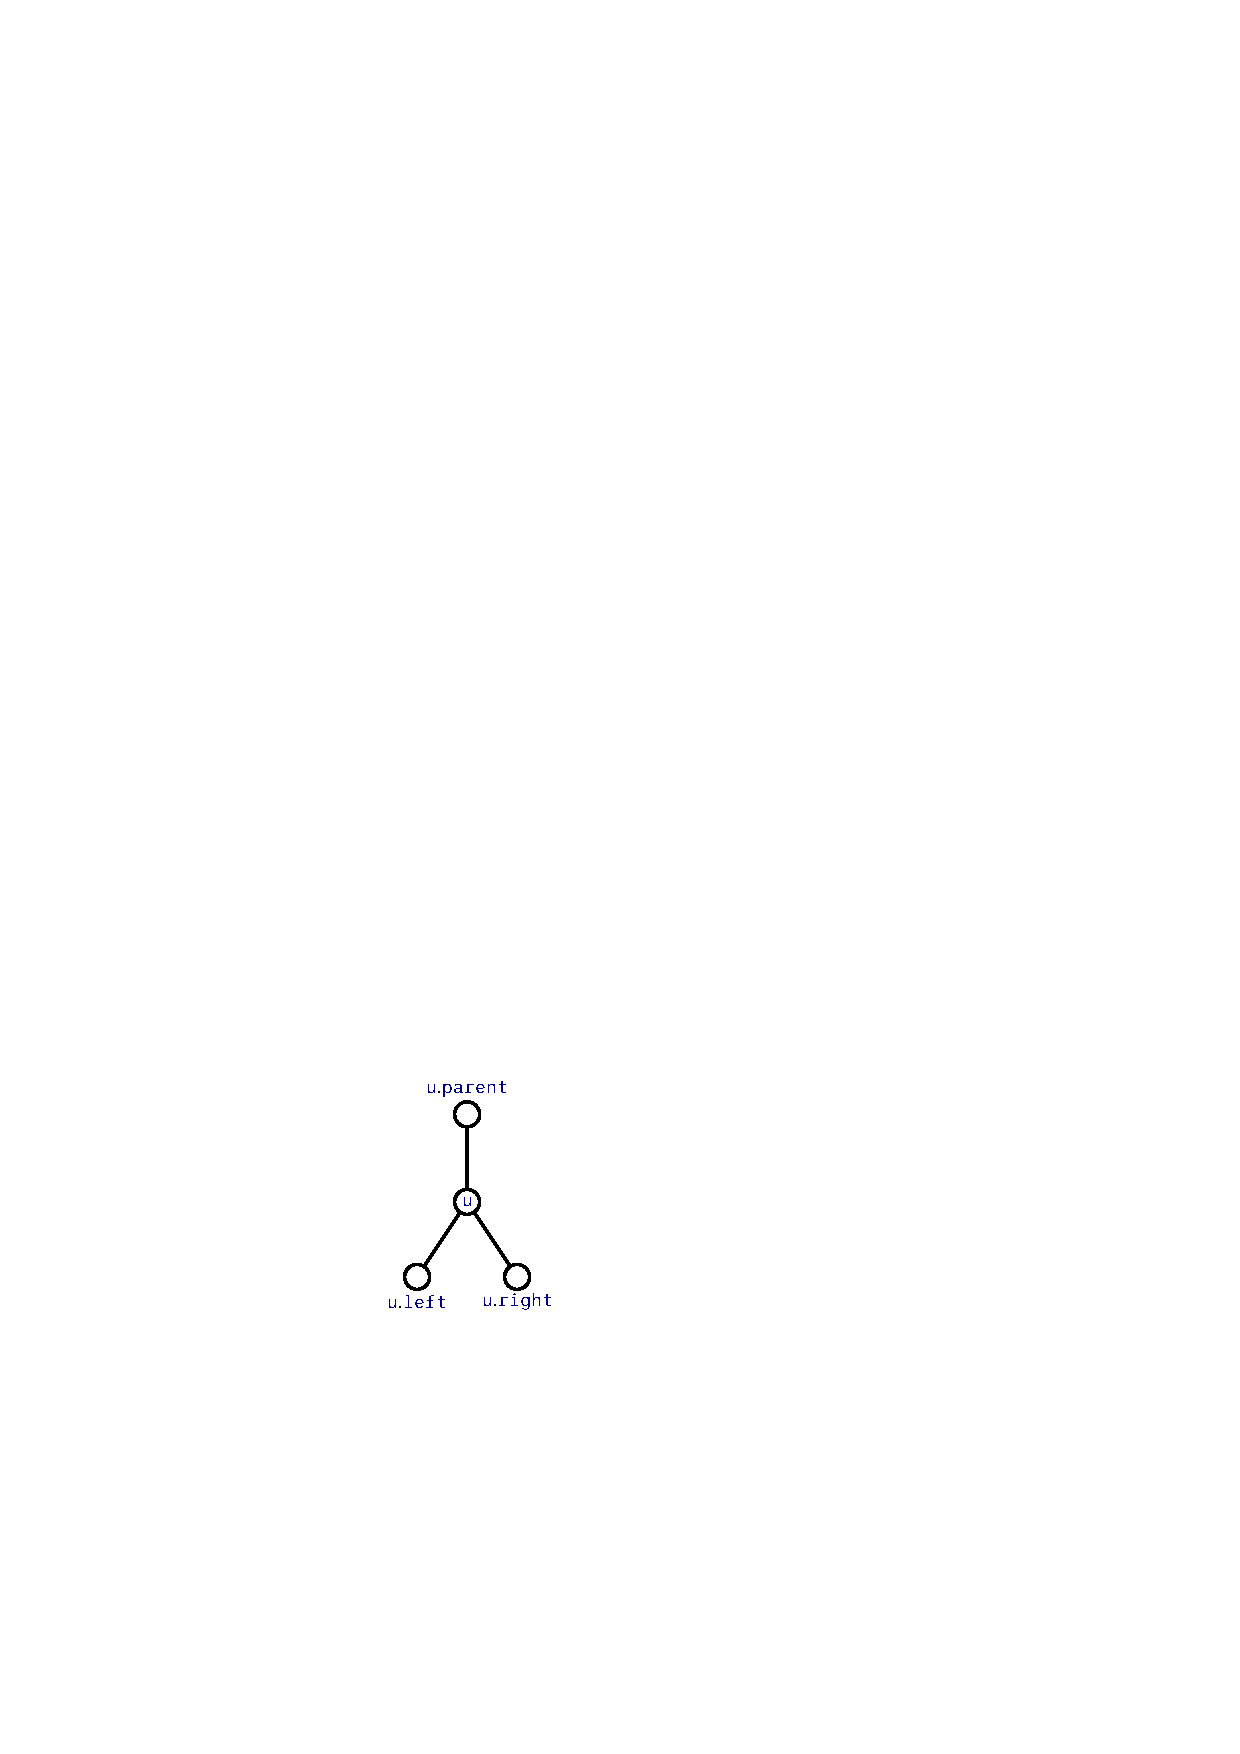
\includegraphics[scale=0.90909]{figs/bintree-traverse-1} 
  \end{center}
  \caption[Parent, left child, and right child]{The parent, left child, and right child of the node #u#
    in a #BinaryTree#.}
  \figlabel{bintree-orientation}
\end{figure}


\begin{figure}
  \begin{center}
    \begin{tabular}{cc}
      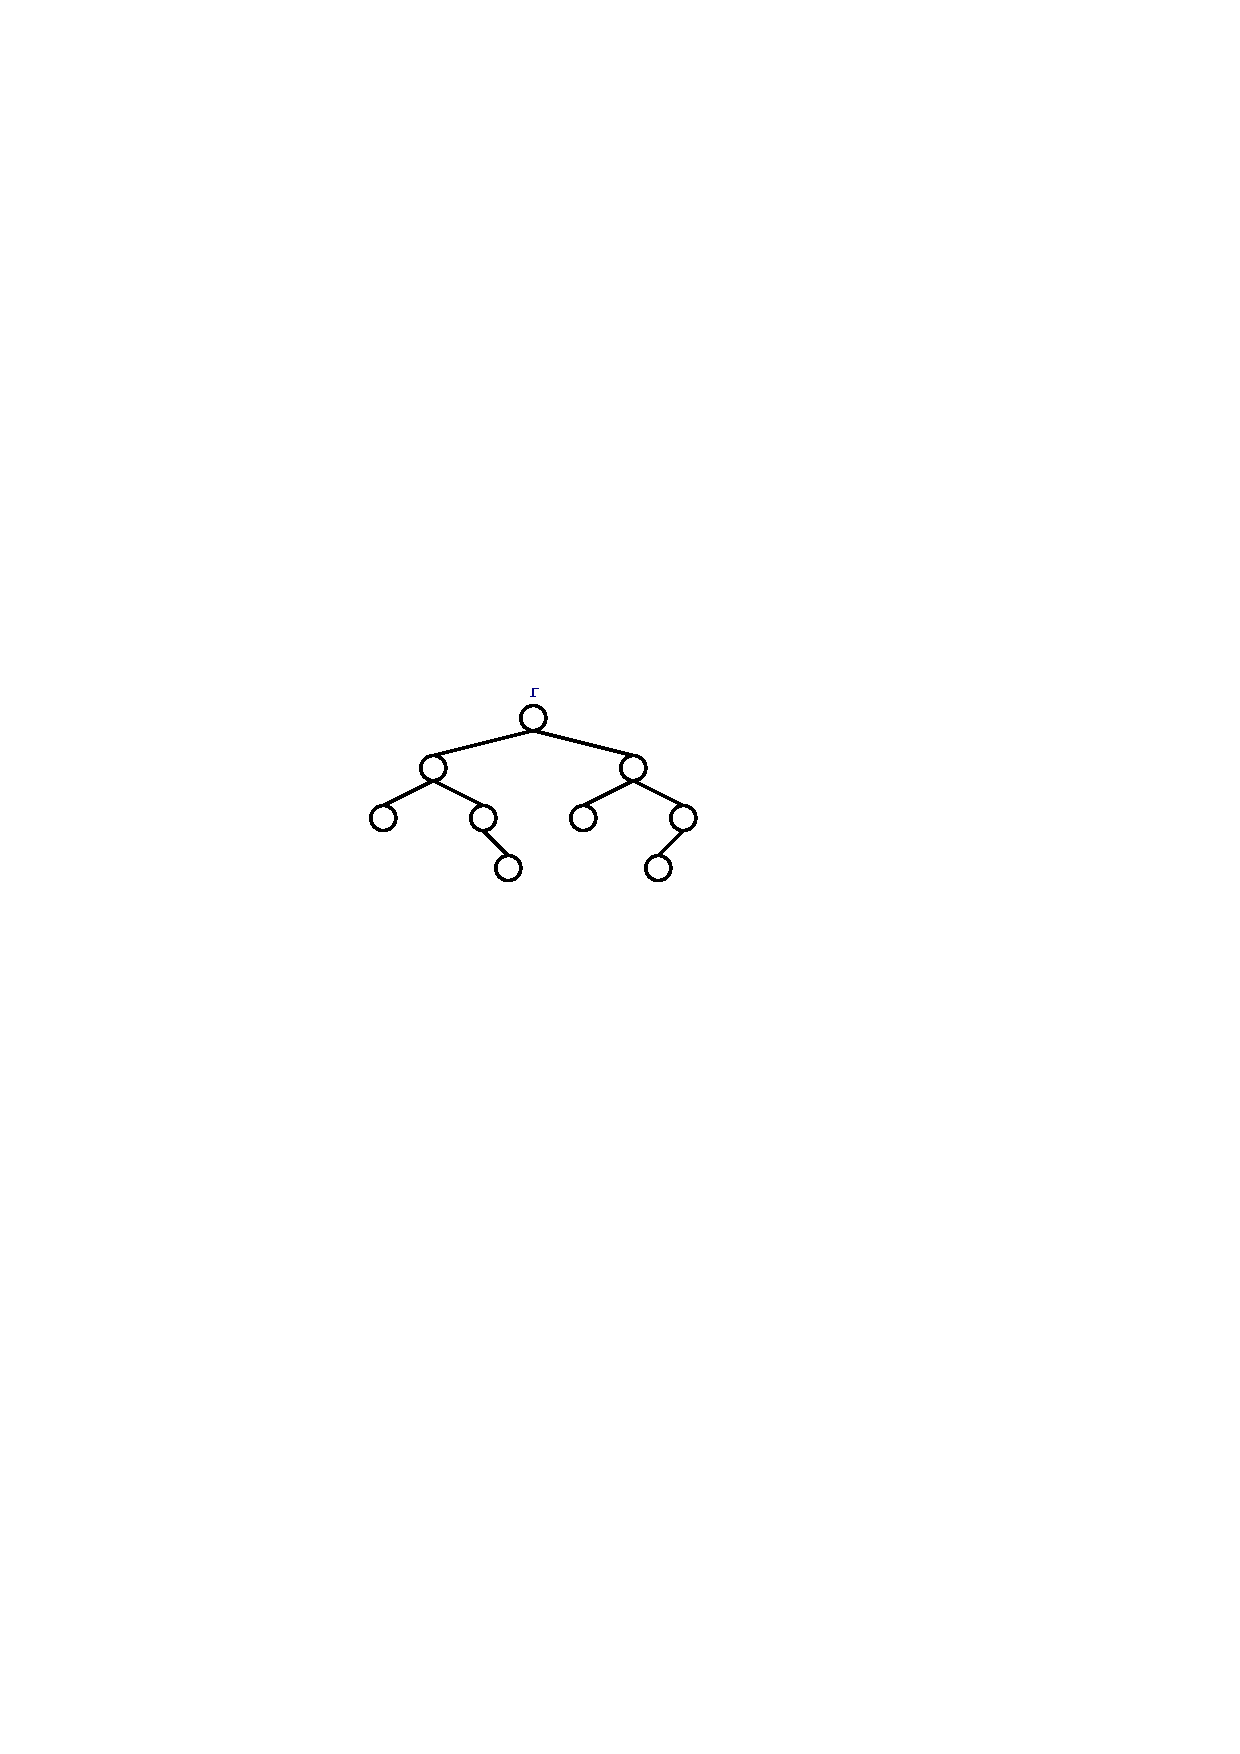
\includegraphics[width=\HalfScaleIfNeeded]{figs/bintree-1} &
      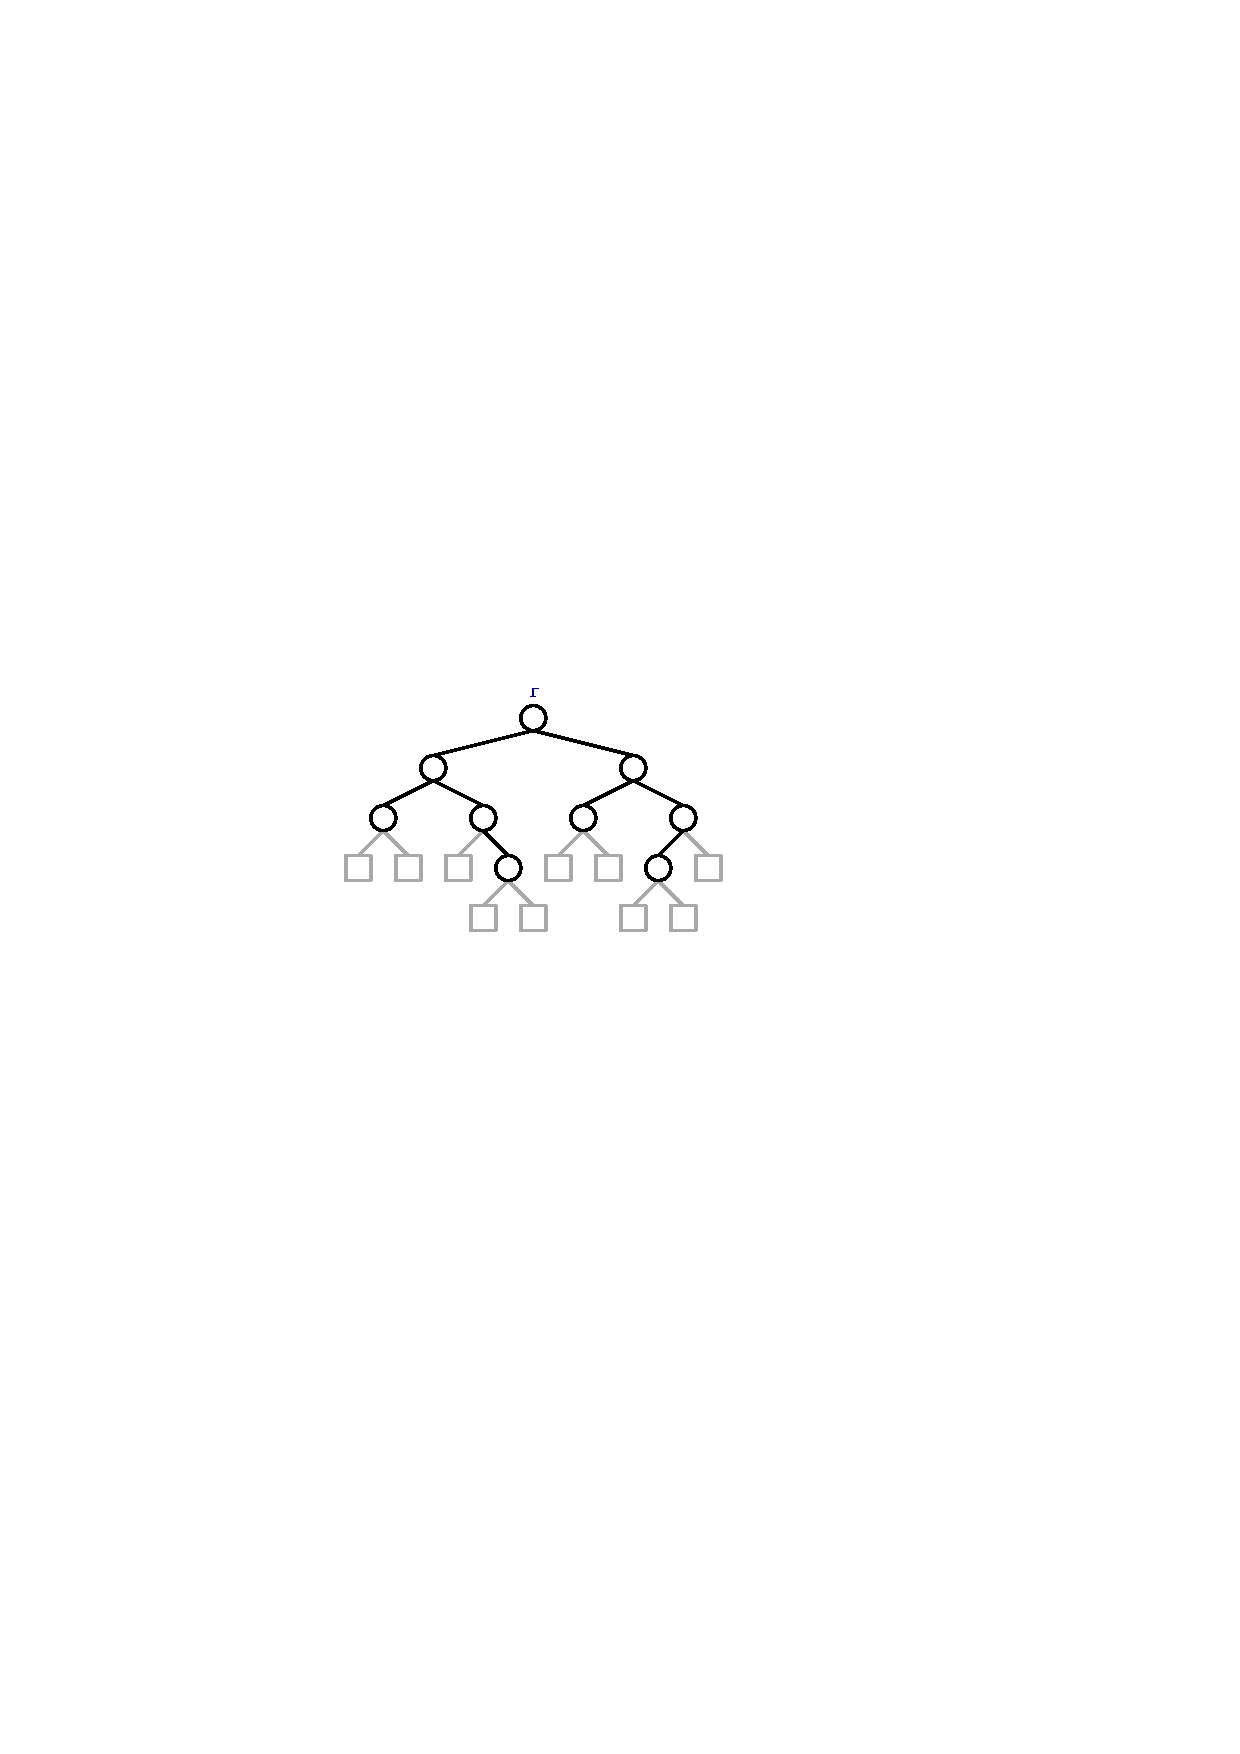
\includegraphics[width=\HalfScaleIfNeeded]{figs/bintree-2} \\
      (a) & (b)
    \end{tabular}
  \end{center}
  \caption{A binary tree with (a)~nine real nodes and (b)~ten external nodes.}
  \figlabel{binary-tree}
\end{figure}

Because binary trees are so important, a certain terminology has developed
for them: The \emph{depth}
\index{depth}%
of a node, #u#, in a binary tree is the
length of the path from #u# to the root of the tree.   If a node, #w#,
is on the path from #u# to #r#, then #w# is called an \emph{ancestor}
\index{ancestor}%
of #u# and #u# a \emph{descendant}
\index{descendant}%
of #w#.  The \emph{subtree} of a
node, #u#, is the binary tree that is rooted at #u# and contains all
of #u#'s descendants.  The \emph{height}
\index{height!in a tree} of a node, #u#, is the length
of the longest path from #u# to one of its descendants.  The \emph{height} of
\index{height!of a tree}%
a tree is the height of its root.
A node, #u#, is a \emph{leaf}
\index{leaf}%
if it has no children.

We sometimes think of the tree as being augmented with \emph{external
nodes}. Any node that does not have a left child has an external
node as its left child, and, correspondingly, any node that does
not have a right child has an external node as its right child (see
\figref{binary-tree}.b).  It is easy to verify, by induction, that a
binary tree with $#n#\ge 1$ real nodes has $#n#+1$ external nodes.


\section{#BinaryTree#: A Basic Binary Tree}

\index{BinaryTree@#BinaryTree#}%
The simplest way to represent a node, #u#, in a binary tree is to
explicitly store the (at most three) neighbours of #u#\notpcode{:}\pcodeonly{.}
\javaimport{ods/BinaryTree.BTNode<Node}
\cppimport{ods/BinaryTree.BTNode}
When one of these three neighbours is not present, we set it to #nil#.
In this way, both external nodes of the tree and the parent of the root
correspond to the value #nil#.

The binary tree itself can then be represented by a
\javaonly{reference}\cpponly{pointer}\pcodeonly{reference} to its root node, #r#:
\codeimport{ods/BinaryTree.r}

We can compute the depth of a node, #u#, in a binary tree by counting
the number of steps on the path from #u# to the root:
\codeimport{ods/BinaryTree.depth(u)}


\subsection{Recursive Algorithms}

\index{recursive algorithm}%
Using recursive algorithms makes it very easy to compute facts about
binary trees. For example, to compute the size of (number of nodes in)
a binary tree rooted at node #u#, we recursively compute the sizes of the
two subtrees rooted at the children of #u#, sum up these sizes, and add one:

\codeimport{ods/BinaryTree.size(u)}

To compute the height of a node #u#, we can compute the height of #u#'s
two subtrees, take the maximum, and add one:

\codeimport{ods/BinaryTree.height(u)}

\subsection{Traversing Binary Trees}
\seclabel{bintree:traversal}

\index{traversal!of a binary tree}%
\index{tree traversal}%
\index{binary-tree traversal}%
The two algorithms from the previous section both use recursion to visit
all the nodes in a binary tree.  Each of them visits the nodes of the
binary tree in the same order as the following code:
\codeimport{ods/BinaryTree.traverse(u)}

Using recursion this way produces very short, simple code, but it can
also be problematic.  The maximum depth of the recursion is given by
the maximum depth of a node in the binary tree, i.e., the tree's height.
If the height of the tree is very large, then this recursion could very
well use more stack space than is available, causing a crash.

To traverse a binary tree without recursion, you can use an algorithm that
relies on where it came from to determine where it will go next.  See
\figref{bintree-traverse}.  If we arrive at a node #u# from #u.parent#,
then the next thing to do is to visit #u.left#.  If we arrive at #u#
from #u.left#, then the next thing to do is to visit #u.right#.  If we
arrive at #u# from #u.right#, then we are done visiting #u#'s subtree,
and so we return to #u.parent#.  The following code implements this
idea, with code included for handling the cases where any of #u.left#,
#u.right#, or #u.parent# is #nil#:
\codeimport{ods/BinaryTree.traverse2()}

\begin{figure}
  \begin{center}
    \begin{tabular}{cc}
      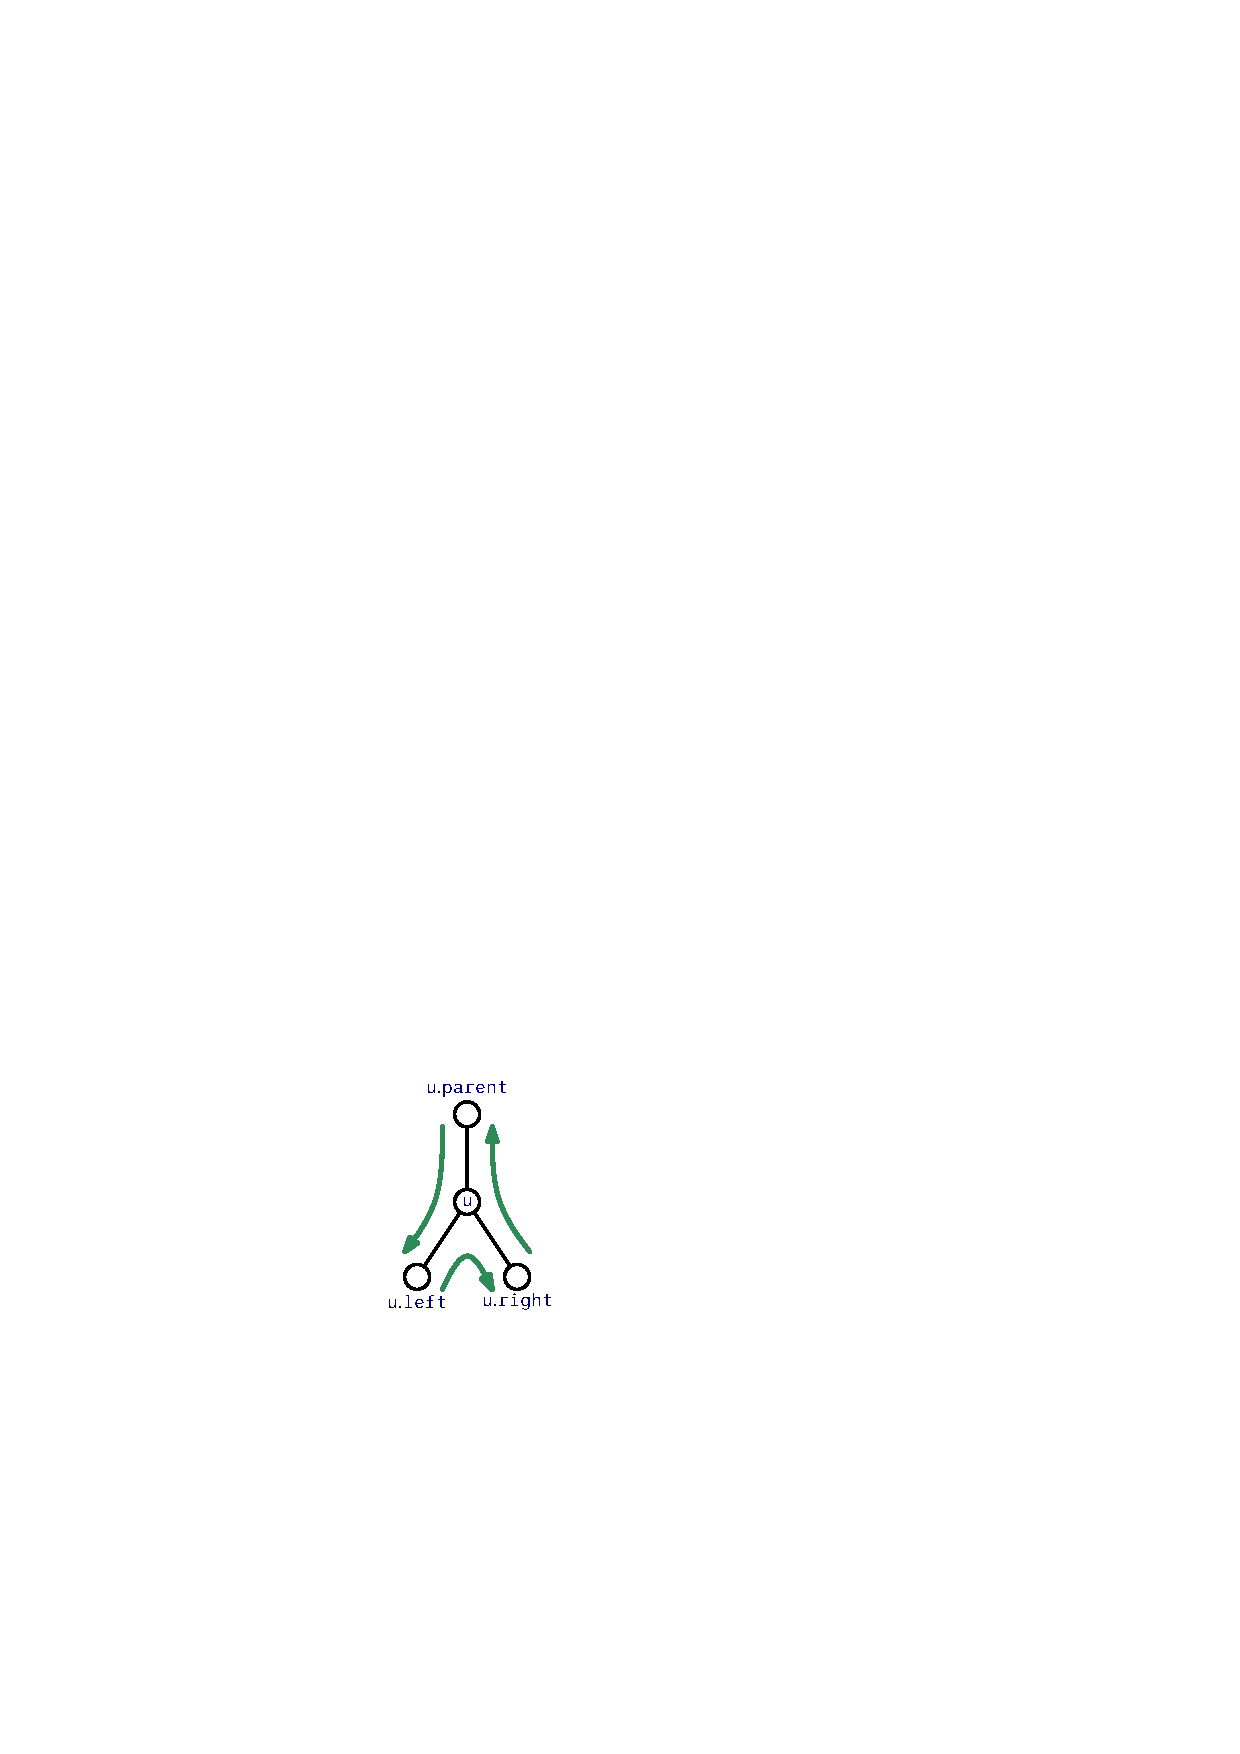
\includegraphics[scale=0.90909]{figs/bintree-traverse-2}
      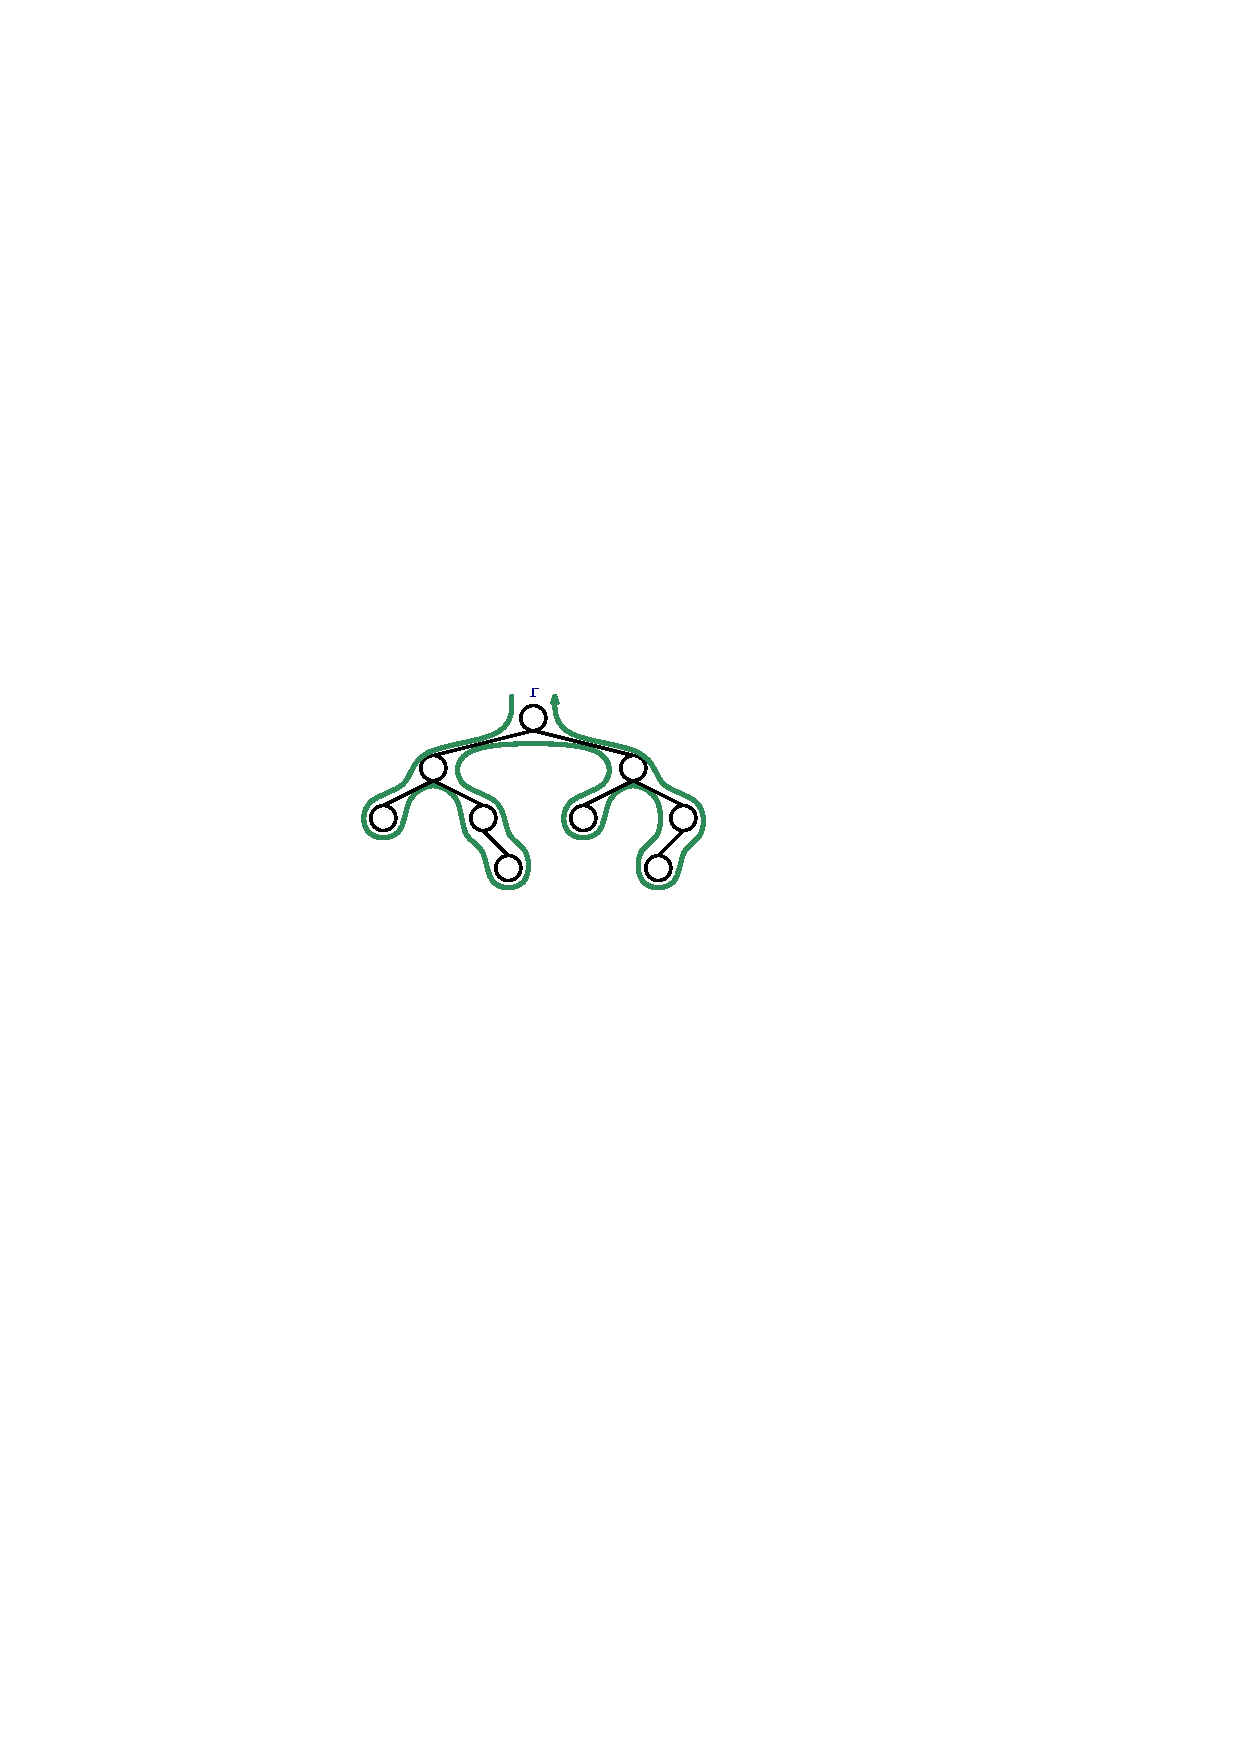
\includegraphics[scale=0.90909]{figs/bintree-3}
    \end{tabular}
  \end{center}
  \caption[Traversing a BinaryTree]{The three cases that occur at node
    #u# when traversing a binary tree non-recursively, and the resultant
    traversal of the tree.}
  \figlabel{bintree-traverse}
\end{figure}

The same facts that can be computed with recursive algorithms can also be
computed in this way, without recursion. For example, to compute the size
of the tree we keep a counter, #n#, and increment #n# whenever visiting
a node for the first time:
\codeimport{ods/BinaryTree.size2()}

In some implementations of binary trees, the #parent# field is not used.
When this is the case, a non-recursive implementation is still possible,
but the implementation has to use a #List# (or #Stack#) to keep track
of the path from the current node to the root.

A special kind of traversal that does not fit the pattern of the above
functions is the \emph{breadth-first traversal}.
\index{breadth-first traversal}%
\index{traversal!breadth-first}%
In a breadth-first
traversal, the nodes are visited level-by-level starting at the root and
moving down, visiting the nodes at each level from left to right (see
\figref{bintree-bfs}). This is similar to the way that we would read a
page of English text.   Breadth-first traversal is implemented using a
queue, #q#, that initially contains only the root, #r#.  At each step,
we extract the next node, #u#, from #q#, process #u# and add #u.left#
and #u.right# (if they are non-#nil#) to #q#:
\codeimport{ods/BinaryTree.bfTraverse()}

\begin{figure}
  \begin{center}
    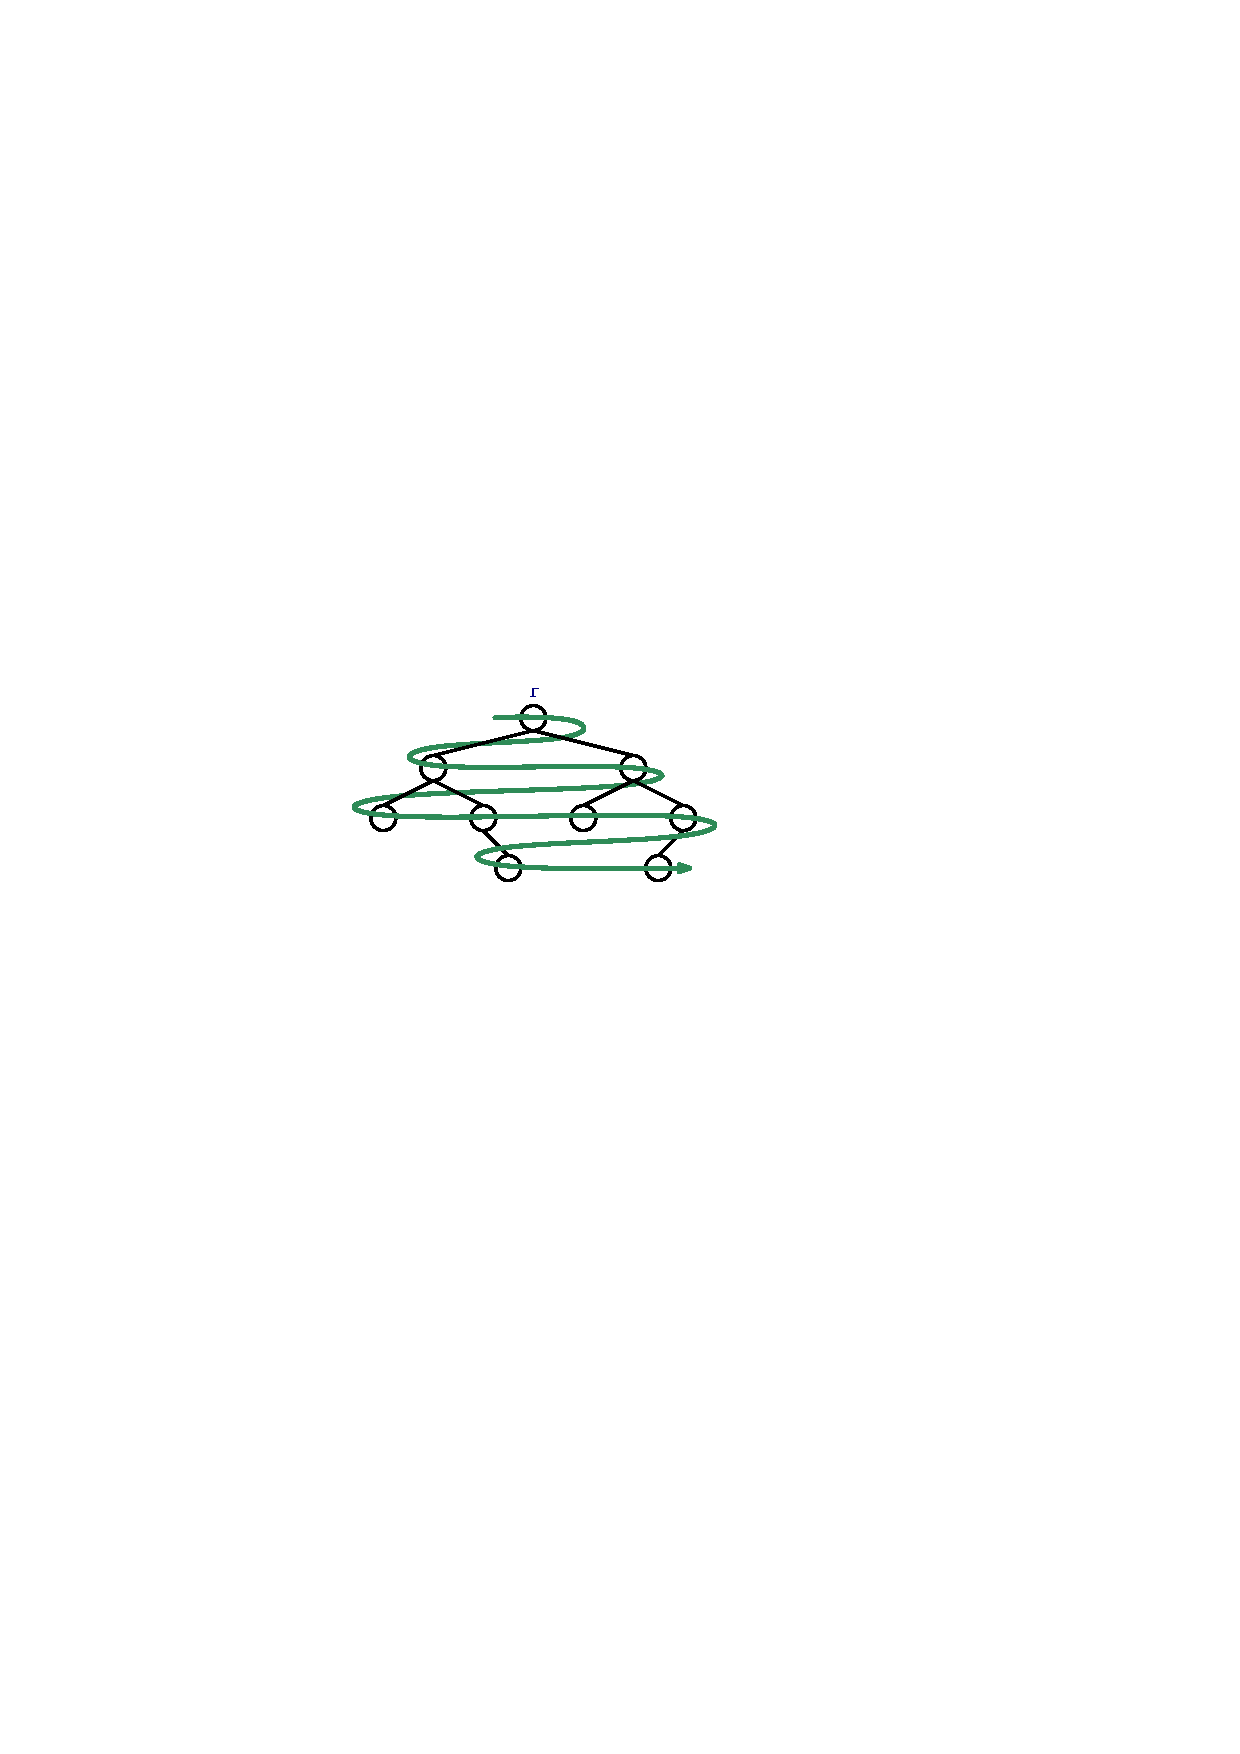
\includegraphics[scale=0.90909]{figs/bintree-4}
  \end{center}
  \caption{During a breadth-first traversal, the nodes of a binary tree
  are visited
level-by-level, and left-to-right within each level.}
  \figlabel{bintree-bfs}
\end{figure}





\section{#BinarySearchTree#: An Unbalanced Binary Search Tree}
\seclabel{binarysearchtree}

\index{BinarySearchTree@#BinarySearchTree#}%
\index{binary search tree}%
\index{binary tree!search}%
A #BinarySearchTree# is a special kind of binary tree in which each node, #u#,
also stores a data value, #u.x#, from some total order.  The data values in
a binary search tree obey the \emph{binary search tree property}:
\index{binary search tree property}%
For
a node, #u#, every data value stored in the subtree rooted at #u.left#
is less than #u.x# and every data value stored in the subtree rooted at
#u.right# is greater than #u.x#.  An example of a #BinarySearchTree# is shown in \figref{bst}.

\begin{figure}
  \begin{center}
    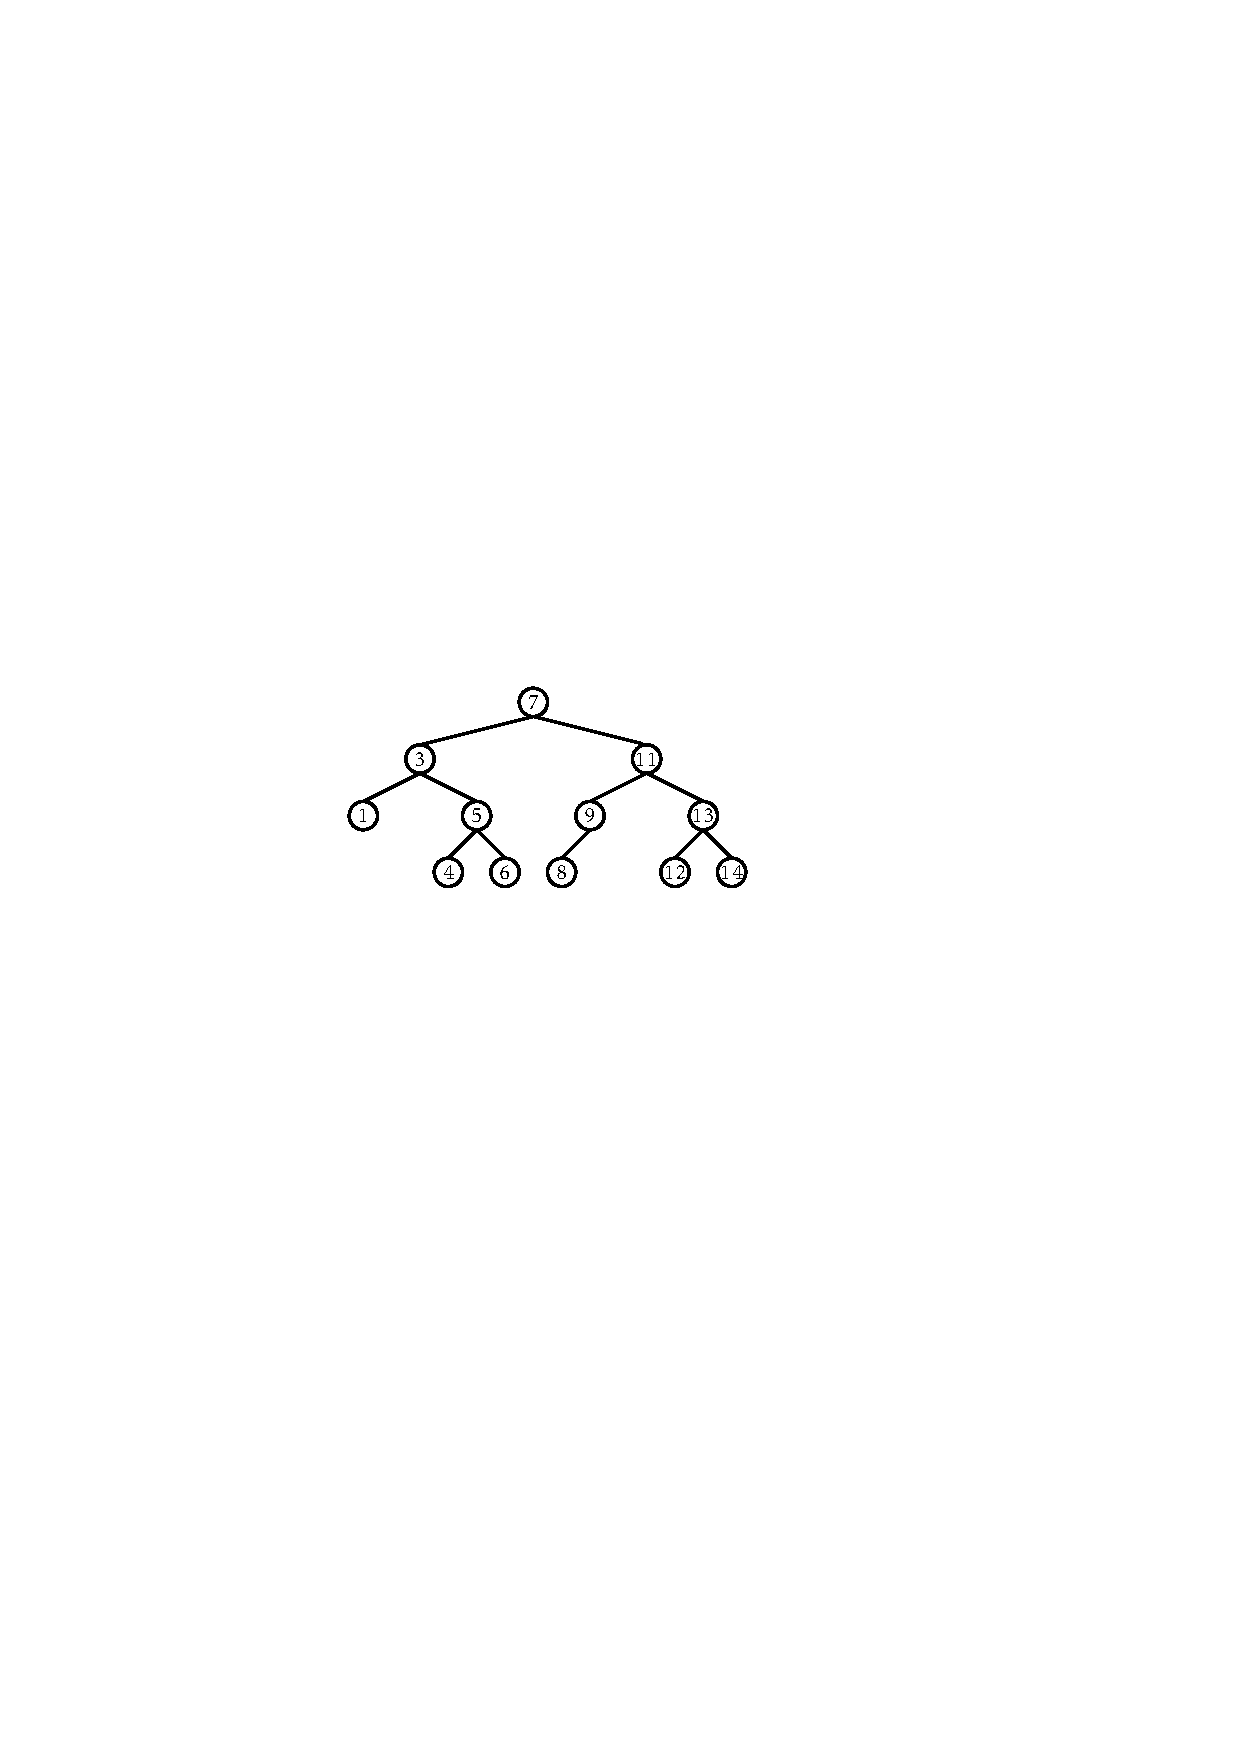
\includegraphics[scale=0.90909]{figs/bst-example}
    %\includegraphics[scale=0.90909]{figs/binary-tree-4}
  \end{center}
  \caption{A binary search tree.}
  \figlabel{bst}
\end{figure}


\subsection{Searching}

\index{search path!in a binary search tree}%
The binary search tree property is extremely useful because it allows
us to quickly locate a value, #x#, in a binary search tree.  To do this we start
searching for #x# at the root, #r#.  When examining a node, #u#, there
are three cases:
\begin{enumerate}
\item If $#x#< #u.x#$, then the search proceeds to #u.left#;
\item If $#x#> #u.x#$, then the search proceeds to #u.right#;
\item If $#x#= #u.x#$, then we have found the node #u# containing #x#.
\end{enumerate}
The search terminates when Case~3 occurs or when #u=nil#.  In the
former case, we found #x#.  In the latter case, we conclude that #x#
is not in the binary search tree.
\codeimport{ods/BinarySearchTree.findEQ(x)}

Two examples of searches in a binary search tree are shown in
\figref{bst-search}.  As the second example shows, even if we don't
find #x# in the tree, we still gain some valuable information.  If we
look at the last node, #u#, at which Case~1 occurred, we see that #u.x#
is the smallest value in the tree that is greater than #x#.  Similarly,
the last node at which Case~2 occurred contains the largest value in the
tree that is less than #x#.  Therefore, by keeping track of the last
node, #z#, at which Case~1 occurs, a #BinarySearchTree# can implement
the #find(x)# operation that returns the smallest value stored in the
tree that is greater than or equal to #x#:
\codeimport{ods/BinarySearchTree.find(x)}

\begin{figure}
  \begin{center}
    \begin{tabular}{cc}
    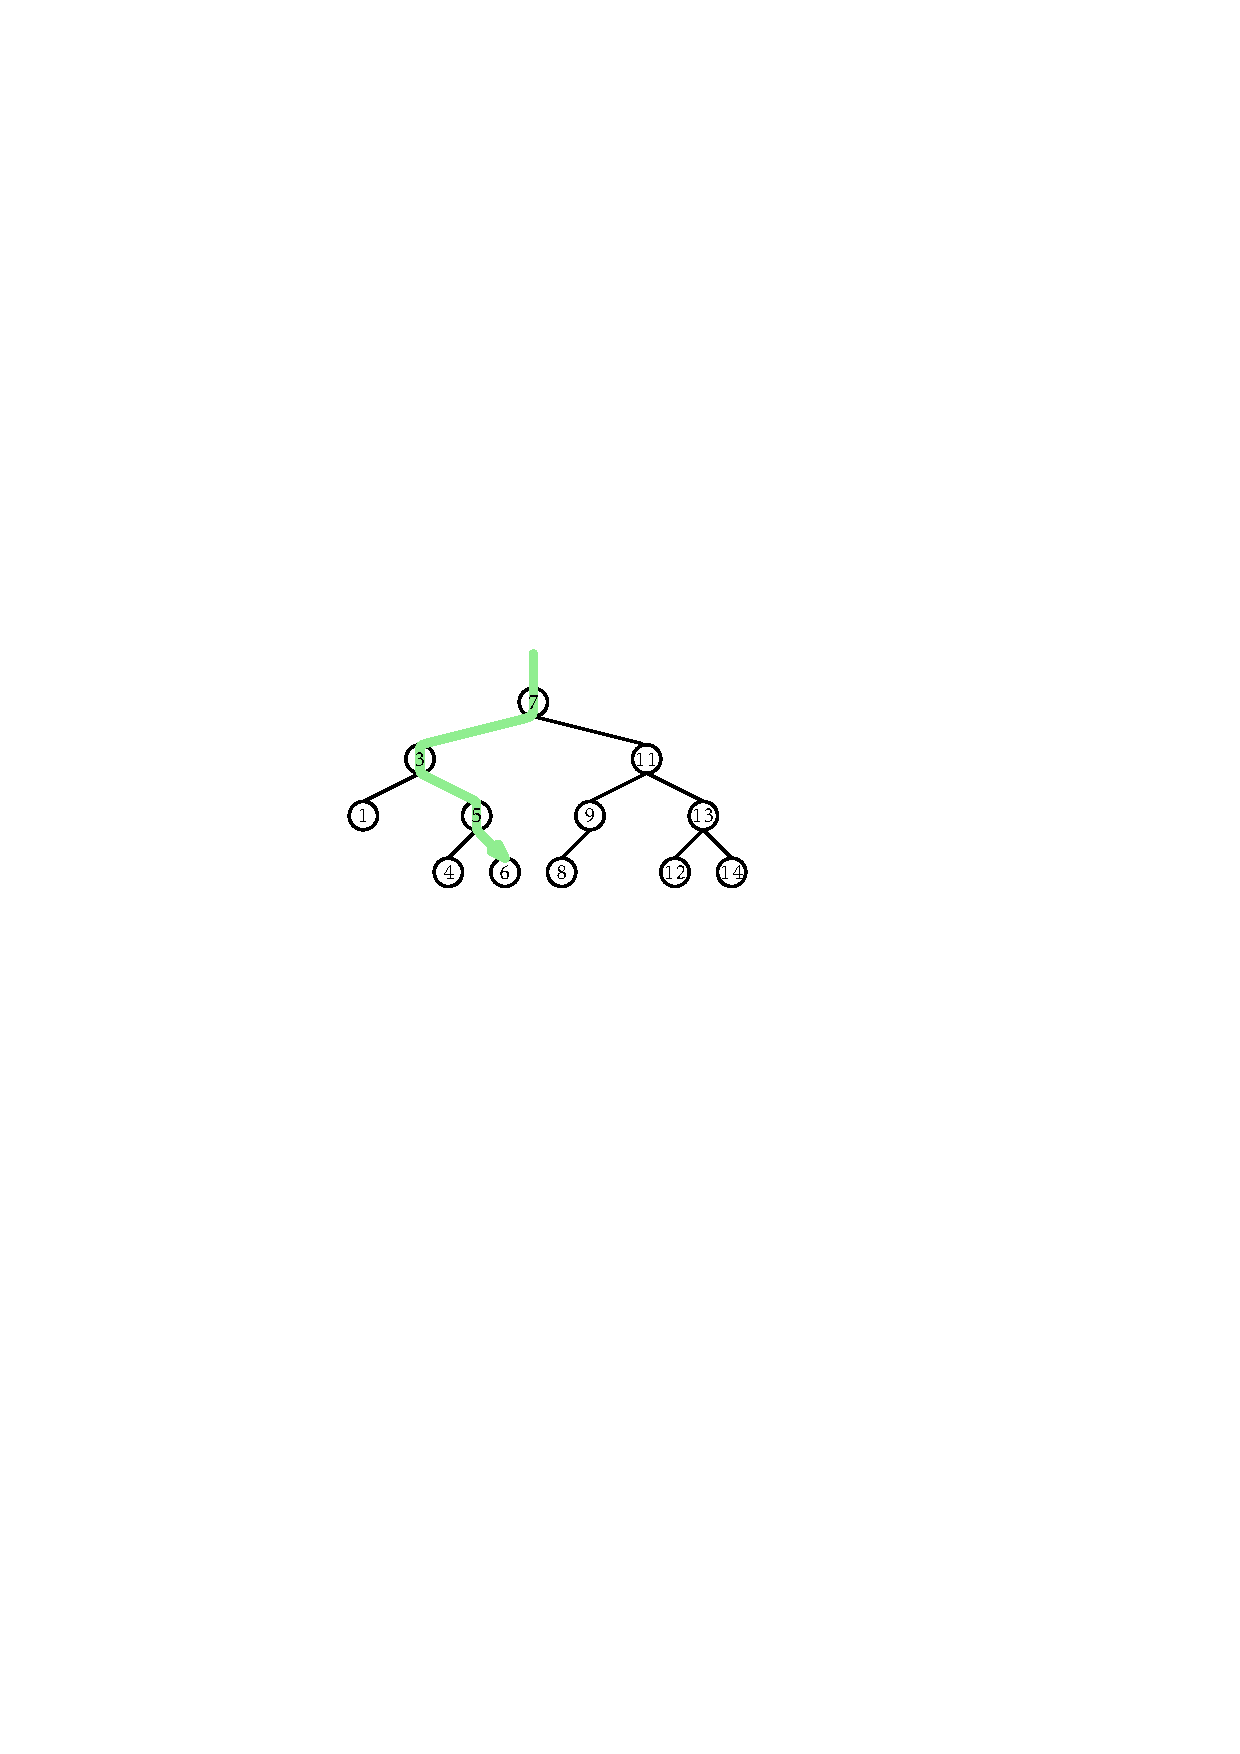
\includegraphics[width=\HalfScaleIfNeeded]{figs/bst-example-2} &
    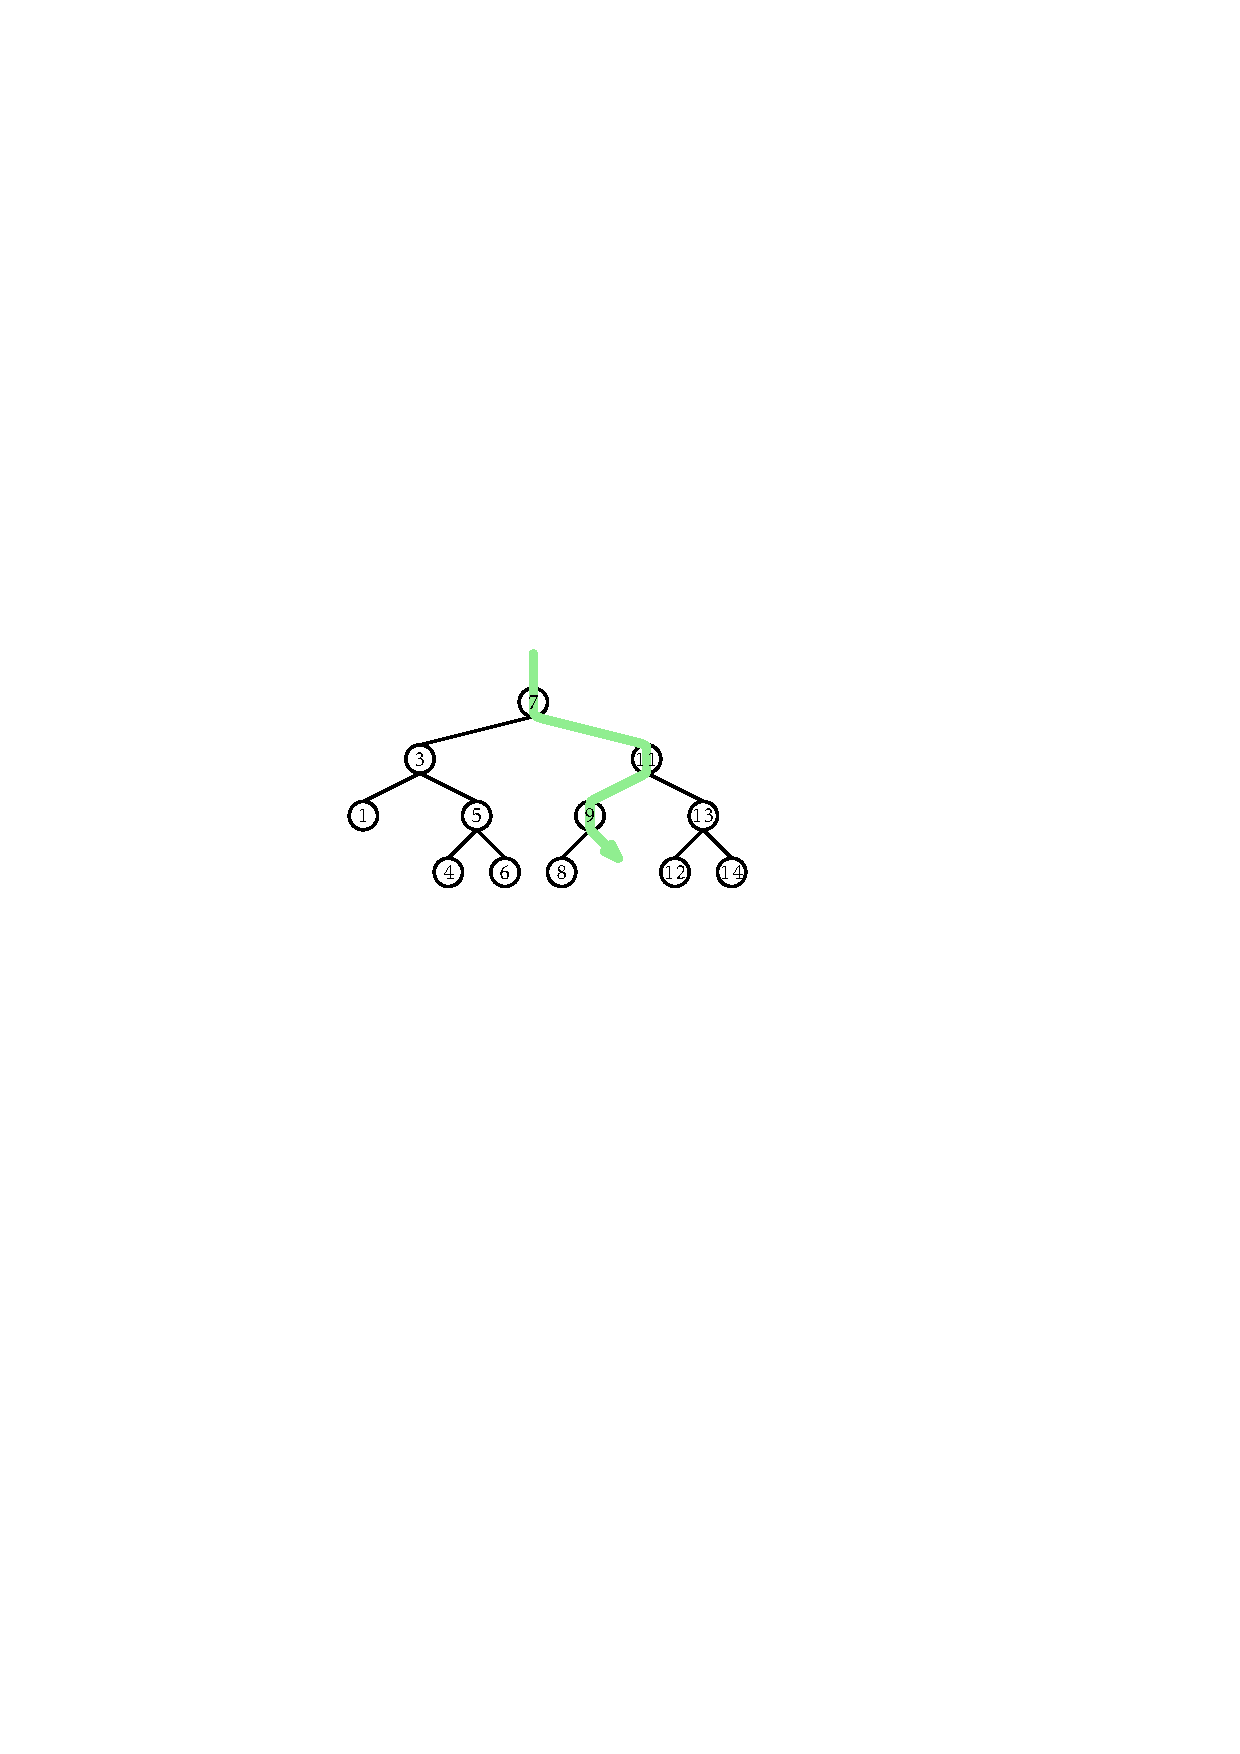
\includegraphics[width=\HalfScaleIfNeeded]{figs/bst-example-3} \\
    (a) & (b)
    \end{tabular}
  \end{center}
  \caption{An example of (a)~a successful search (for $6$) and (b)~an unsuccessful search (for $10$) in a binary search tree.}
  \figlabel{bst-search}
\end{figure}


\subsection{Addition}

To add a new value, #x#, to a #BinarySearchTree#, we first search for
#x#. If we find it, then there is no need to insert it.  Otherwise,
we store #x# at a leaf child of the last node, #p#, encountered during the
search for #x#. Whether the new node is the left or right child of #p# depends on the result of comparing #x# and #p.x#.
\codeimport{ods/BinarySearchTree.add(x)}
\codeimport{ods/BinarySearchTree.findLast(x)}
\codeimport{ods/BinarySearchTree.addChild(p,u)}
An example is shown in \figref{bst-insert}. The most time-consuming
part of this process is the initial search for #x#, which takes an
amount of time proportional to the height of the newly added node #u#.
In the worst case, this is equal to the height of the #BinarySearchTree#.


\begin{figure}
  \begin{center}
    \begin{tabular}{cc}
    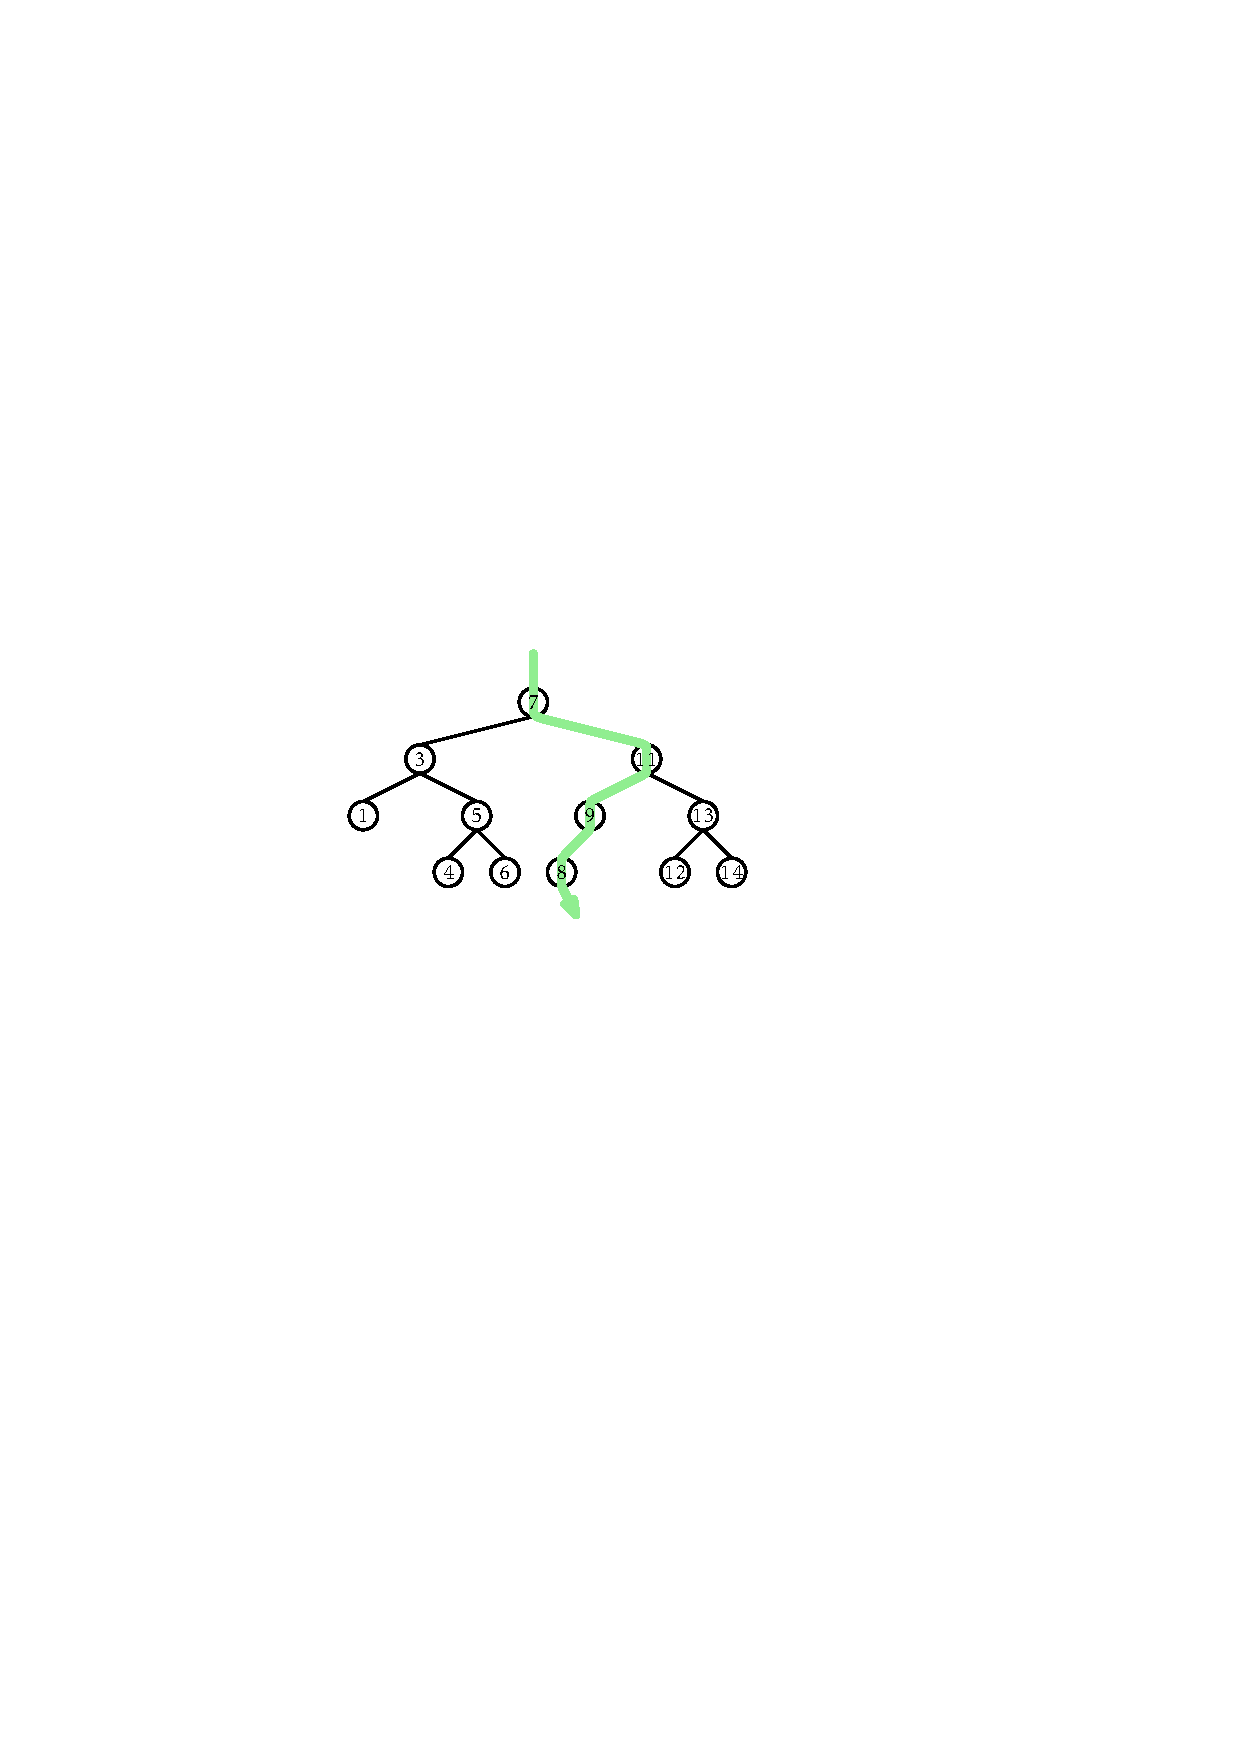
\includegraphics[width=\HalfScaleIfNeeded]{figs/bst-example-4} &
    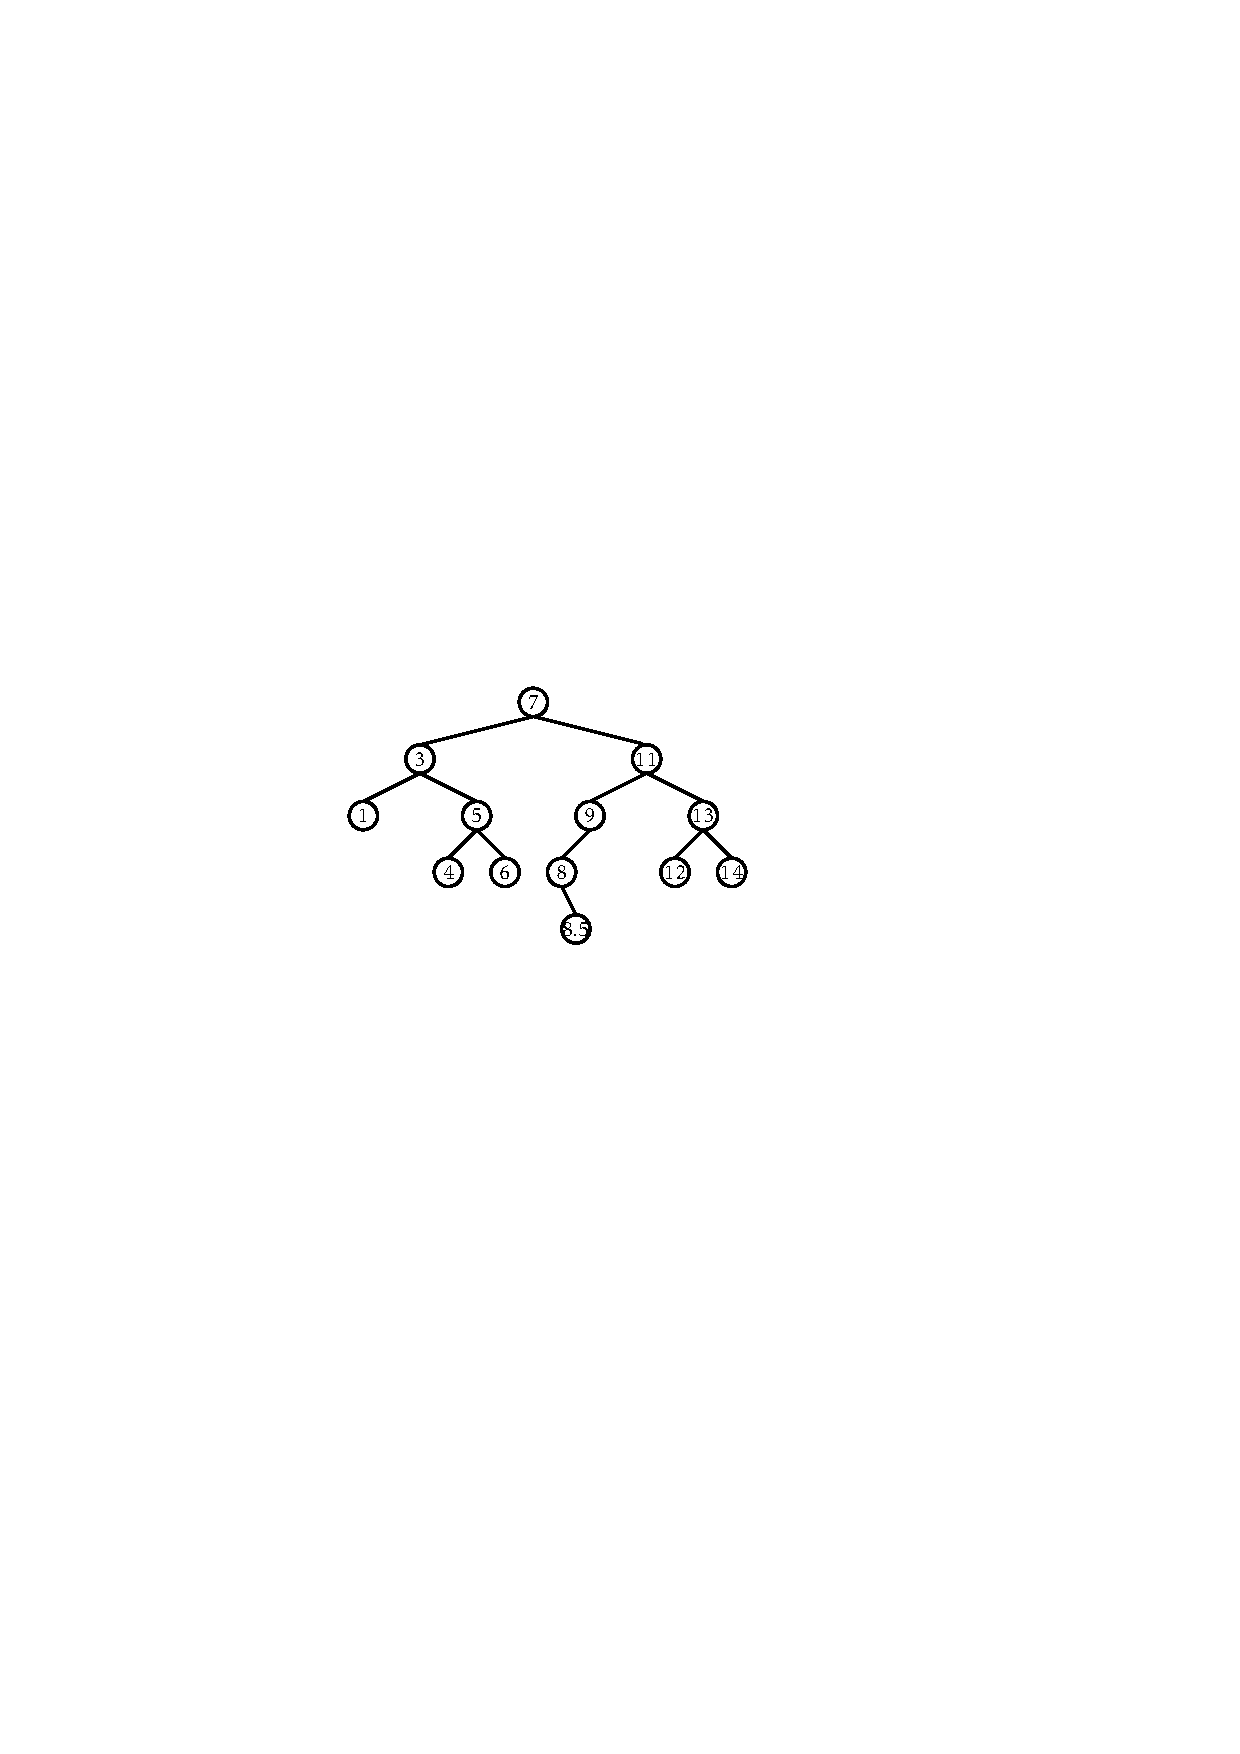
\includegraphics[width=\HalfScaleIfNeeded]{figs/bst-example-5} 
    \end{tabular}
  \end{center}
  \caption{Inserting the value $8.5$ into a binary search tree.}
  \figlabel{bst-insert}
\end{figure}


\subsection{Removal}

Deleting a value stored in a node, #u#, of a #BinarySearchTree# is a
little more difficult.  If #u# is a leaf, then we can just detach #u#
from its parent.  Even better: If #u# has only one child, then we can
splice #u# from the tree by having #u.parent# adopt #u#'s child (see
\figref{bst-splice}):
\codeimport{ods/BinarySearchTree.splice(u)}

\begin{figure}
  \begin{center}
    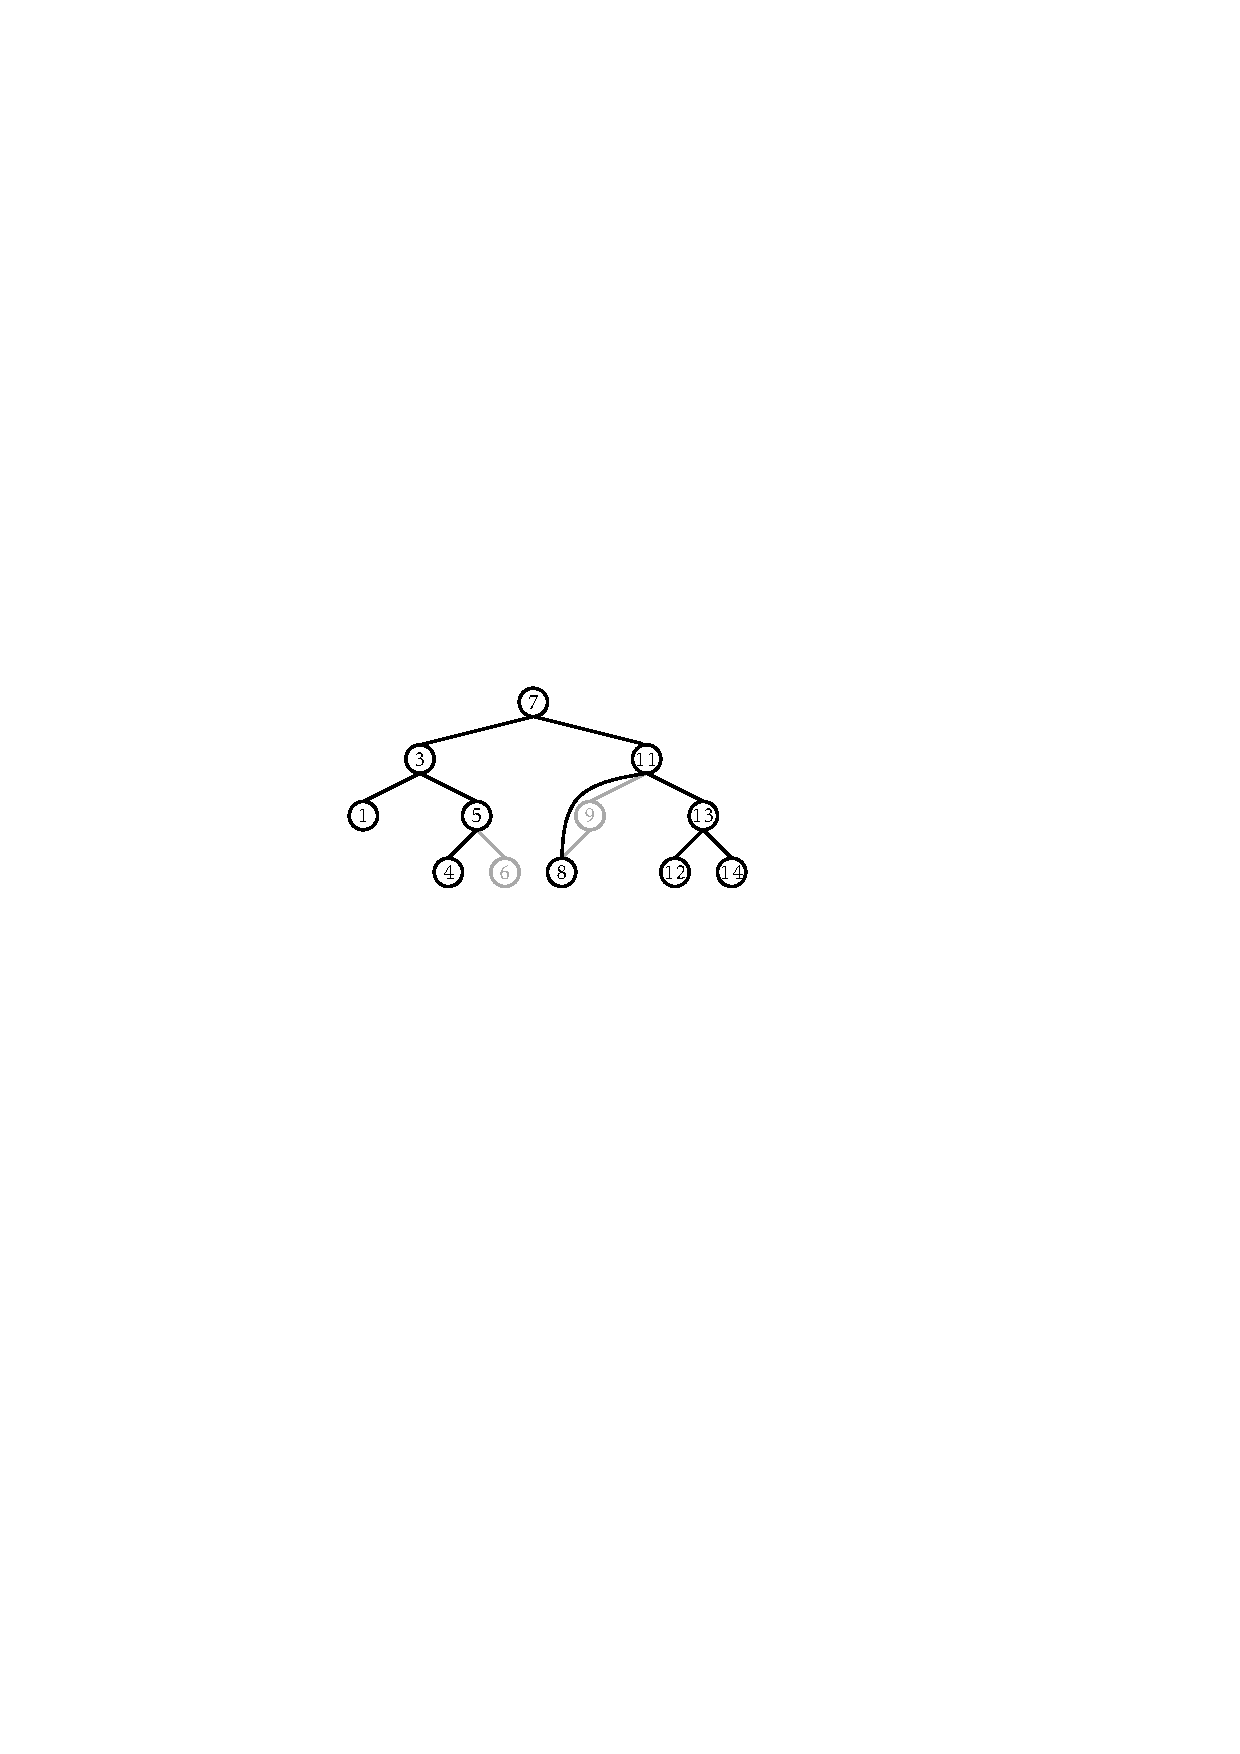
\includegraphics[scale=0.90909]{figs/bst-splice}
  \end{center}
  \caption{Removing a leaf ($6$) or a node with only one child ($9$) is easy.}
  \figlabel{bst-splice}
\end{figure}

Things get tricky, though, when #u# has two children.  In this case,
the simplest thing to do is to find a node, #w#, that has less than
two children and such that #w.x# can replace #u.x#.  To maintain
the binary search tree property, the value #w.x# should be close to the
value of #u.x#.  For example, choosing #w# such that #w.x# is the smallest
value greater than #u.x# will work.  Finding the node #w# is easy; it is
the smallest value in the subtree rooted at #u.right#.  This node can
be easily removed because it has no left child (see \figref{bst-remove}).
\javaimport{ods/BinarySearchTree.remove(u)}
\cppimport{ods/BinarySearchTree.remove(u)}
\pcodeimport{ods/BinarySearchTree.remove_node(u)}

\begin{figure}
  \begin{center}
    \begin{tabular}{cc}
    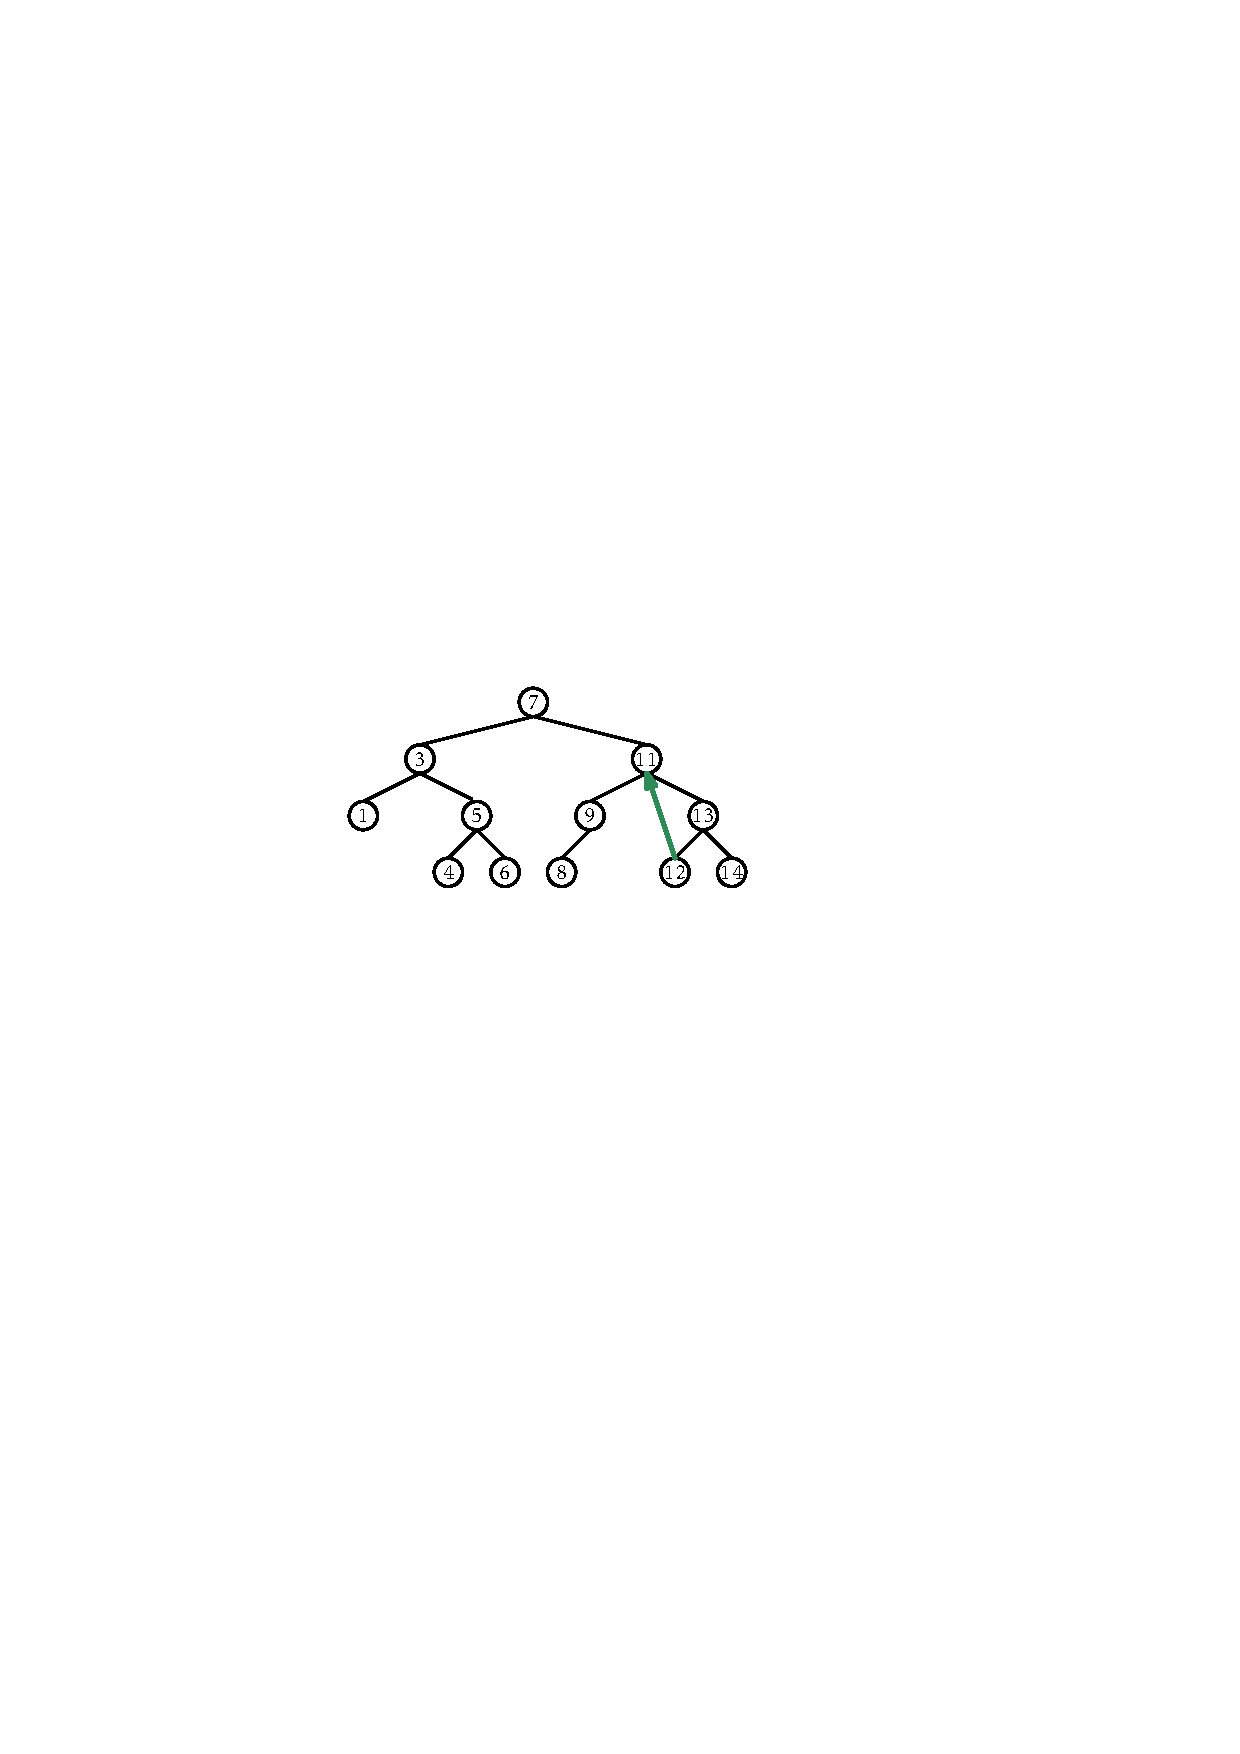
\includegraphics[width=\HalfScaleIfNeeded]{figs/bst-delete-1}
    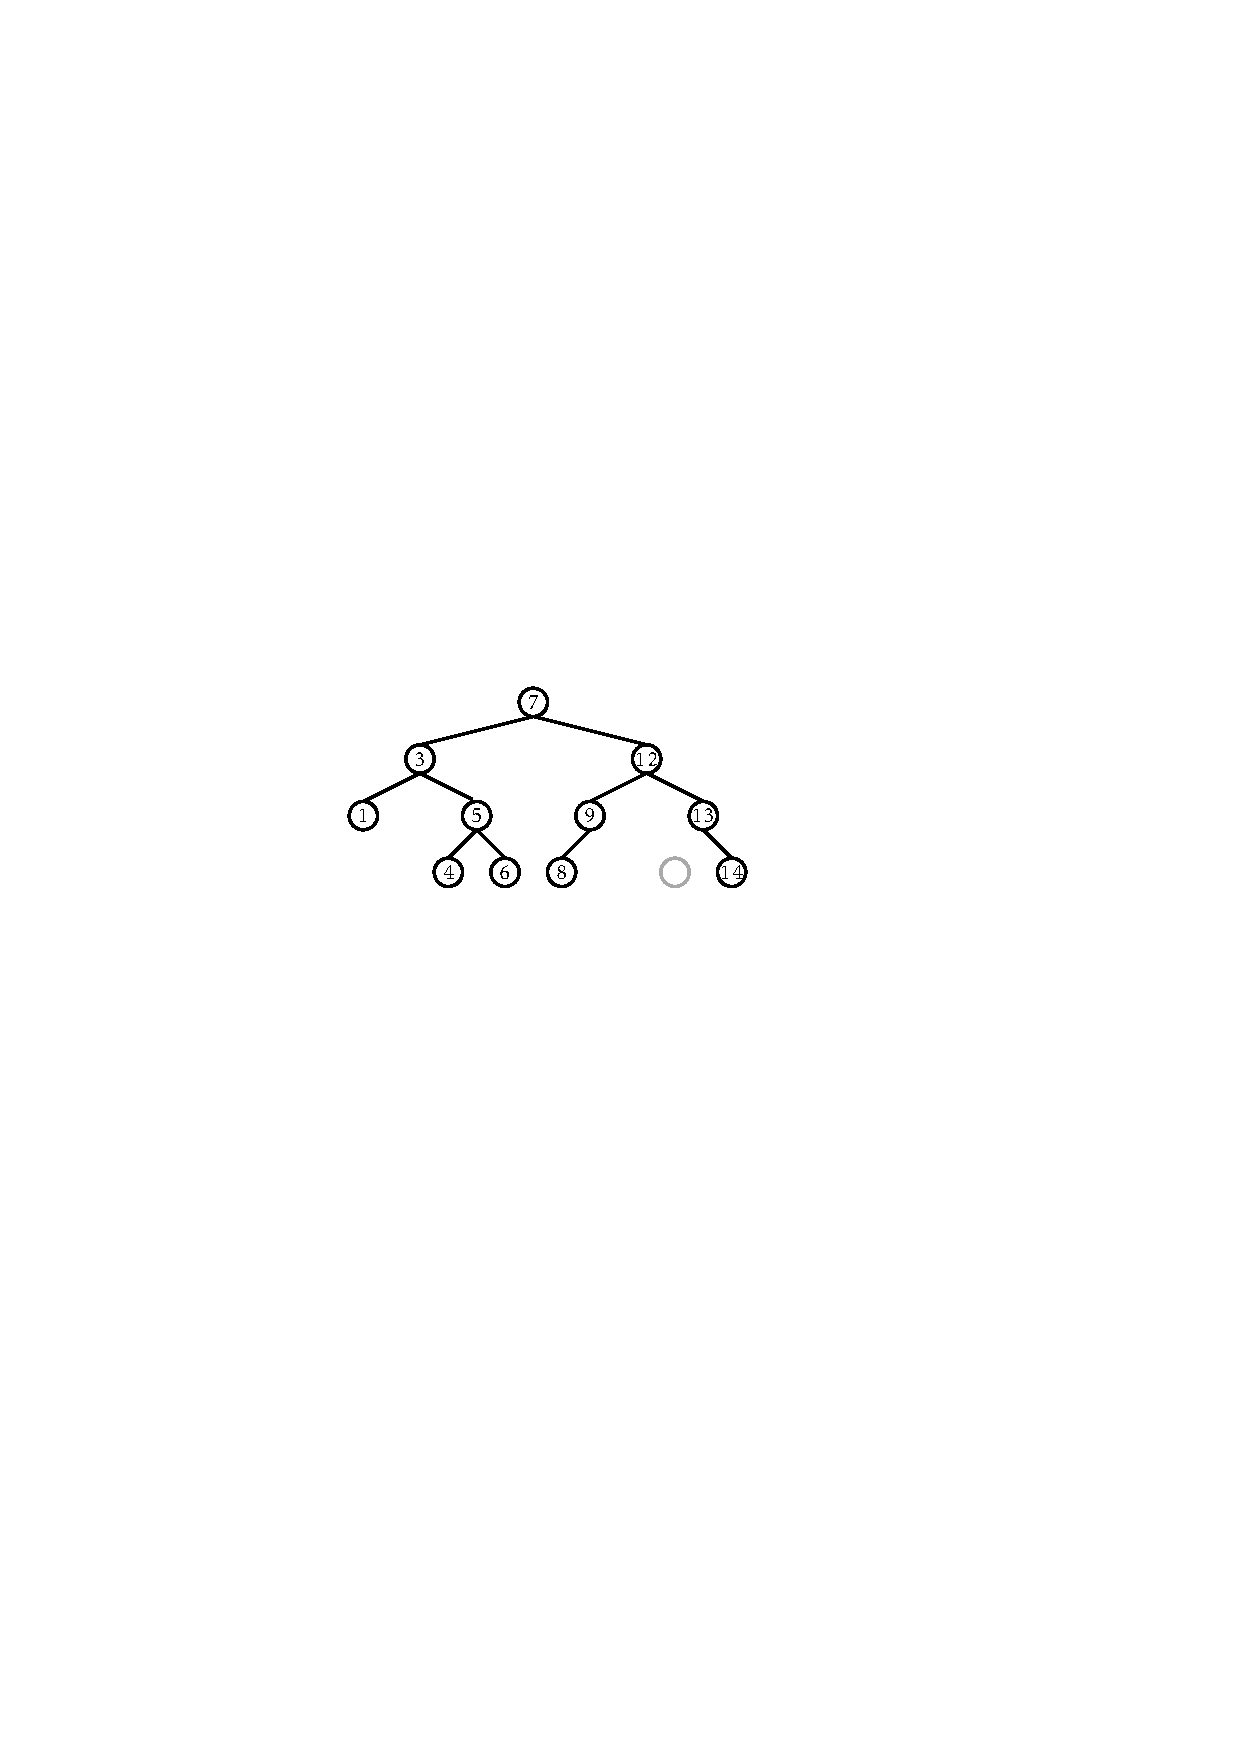
\includegraphics[width=\HalfScaleIfNeeded]{figs/bst-delete-2}
    \end{tabular}
  \end{center}
  \caption[Deleting from a BinarySearchTree]{Deleting a value ($11$) from a node, #u#, with two children is done by replacing #u#'s value with the smallest value in the right subtree of #u#.}
  \figlabel{bst-remove}
\end{figure}

\subsection{Summary}

The #find(x)#, #add(x)#, and #remove(x)# operations in a
#BinarySearchTree# each involve following a path from the root of the
tree to some node in the tree. Without knowing more about the shape of
the tree it is difficult to say much about the length of this path,
except that it is less than #n#, the number of nodes in the tree.
The following (unimpressive) theorem summarizes the performance of the
#BinarySearchTree# data structure:

\begin{thm}\thmlabel{bst}
  #BinarySearchTree# implements the #SSet# interface and 
  supports the operations #add(x)#, #remove(x)#,
  and #find(x)# in $O(#n#)$ time per operation.
\end{thm}

\thmref{bst} compares poorly with \thmref{skiplist}, which shows
that the #SkiplistSSet# structure can implement the #SSet# interface
with $O(\log #n#)$ expected time per operation.  The problem with the
#BinarySearchTree# structure is that it can become \emph{unbalanced}.
Instead of looking like the tree in \figref{bst} it can look like a long
chain of #n# nodes, all but the last having exactly one child.

There are a number of ways of avoiding unbalanced binary search
trees, all of which lead to data structures that have $O(\log
#n#)$ time operations. In \chapref{rbs} we show how $O(\log #n#)$
\emph{expected} time operations can be achieved with randomization.
In \chapref{scapegoat} we show how $O(\log #n#)$ \emph{amortized}
time operations can be achieved with partial rebuilding operations.
In \chapref{redblack} we show how $O(\log #n#)$ \emph{worst-case}
time operations can be achieved by simulating a tree that is not binary:
one in which nodes can have up to four children.

\section{Discussion and Exercises}

Binary trees have been used to model relationships for thousands
of years.  One reason for this is that binary trees naturally model
(pedigree) family trees.
\index{family tree}%
\index{pedigree family tree}%
These are the family trees in which the root is
a person, the left and right children are the person's parents, and so
on, recursively.  In more recent centuries binary trees have also been
used to model species trees
\index{species tree} in biology, where the leaves of the tree
represent extant species and the internal nodes of the tree represent
\emph{speciation events}
\index{speciation event} in which two populations of a single species
evolve into two separate species.

Binary search trees appear to have been discovered independently by
several groups in the 1950s \cite[Section~6.2.2]{k97v3}.  Further
references to specific kinds of binary search trees are provided in
subsequent chapters.

When implementing a binary tree from scratch, there are several design
decisions to be made.  One of these is the question of whether or not
each node stores a pointer to its parent.  If most of the operations
simply follow a root-to-leaf path, then parent pointers are unnecessary,
waste space, and are a potential source of coding errors.  On the other
hand, the lack of parent pointers means that tree traversals must be done
recursively or with the use of an explicit stack.  Some other methods
(like inserting or deleting into some kinds of balanced binary search
trees) are also complicated by the lack of parent pointers.

Another design decision is concerned with how to store the parent, left
child, and right child pointers at a node.  In the implementation given
here, these pointers are stored as separate variables.   Another option
is to store them in an array, #p#, of length 3, so that #u.p[0]# is the
left child of #u#, #u.p[1]# is the right child of #u#, and #u.p[2]# is
the parent of #u#.  Using an array this way means that some sequences
of #if# statements can be simplified into algebraic expressions.

An example of such a simplification occurs during tree traversal. If
a traversal arrives at a node #u# from #u.p[i]#, then the next node in
the traversal is $#u.p#[(#i#+1)\bmod 3]$.  Similar examples occur when
there is left-right symmetry.  For example, the sibling of #u.p[i]# is
$#u.p#[(#i#+1)\bmod 2]$.  This trick works whether #u.p[i]# is a left
child ($#i#=0$) or a right child ($#i#=1$) of #u#.  In some cases this
means that some complicated code that would otherwise need to have both a
left version and right version can be written only once. See the methods
#rotateLeft(u)# and #rotateRight(u)# on page~\pageref{page:rotations}
for an example.

\begin{exc}
  Prove that a binary tree having $#n#\ge 1$ nodes has $#n#-1$ edges.
\end{exc}

\begin{exc}
  Prove that a binary tree having $#n#\ge 1$ real nodes has $#n#+1$
  external nodes.
\end{exc}

\begin{exc}
  Prove that, if a binary tree, $T$, has at least one leaf, then either
  (a)~$T$'s root has at most one child or (b)~$T$ has more than
  one leaf.
\end{exc}

\begin{exc}
  Implement a non-recursive method, #size2(u)#, that computes the size
  of the subtree rooted at node #u#.
\end{exc}

\begin{exc}
  Write a non-recursive method, #height2(u)#, that computes the height
  of node #u# in a #BinaryTree#.
\end{exc}

\begin{exc}
  A binary tree is \emph{size-balanced}
  \index{size-balanced}%
  \index{binary search tree!size-balanced}%
  if, for every node #u#, the size of
  the subtrees rooted at #u.left# and #u.right# differ by at most one.
  Write a recursive method, #isBalanced()#, that tests if a binary tree
  is balanced.  Your method should run in $O(#n#)$ time.  (Be sure to
  test your code on some large trees with different shapes; it is easy
  to write a method that takes much longer than $O(#n#)$ time.)
\end{exc}

\index{traversal!pre-order}%
\index{traversal!post-order}%
\index{traversal!in-order}%
\index{pre-order traversal}%
\index{post-order traversal}%
\index{in-order traversal}%
A \emph{pre-order} traversal of a binary tree is a traversal that visits
each node, #u#, before any of its children.  An \emph{in-order} traversal
visits #u# after visiting all the nodes in #u#'s left subtree but before
visiting any of the nodes in #u#'s right subtree.  A \emph{post-order}
traversal visits #u# only after visiting all other nodes in #u#'s subtree.
The pre/in/post-order numbering of a tree labels the nodes of a tree with
the integers $0,\ldots,#n#-1$ in the order that they are encountered
by a pre/in/post-order traversal.  See \figref{binarytree-numbering}
for an example.

\begin{figure}
  \begin{center}
    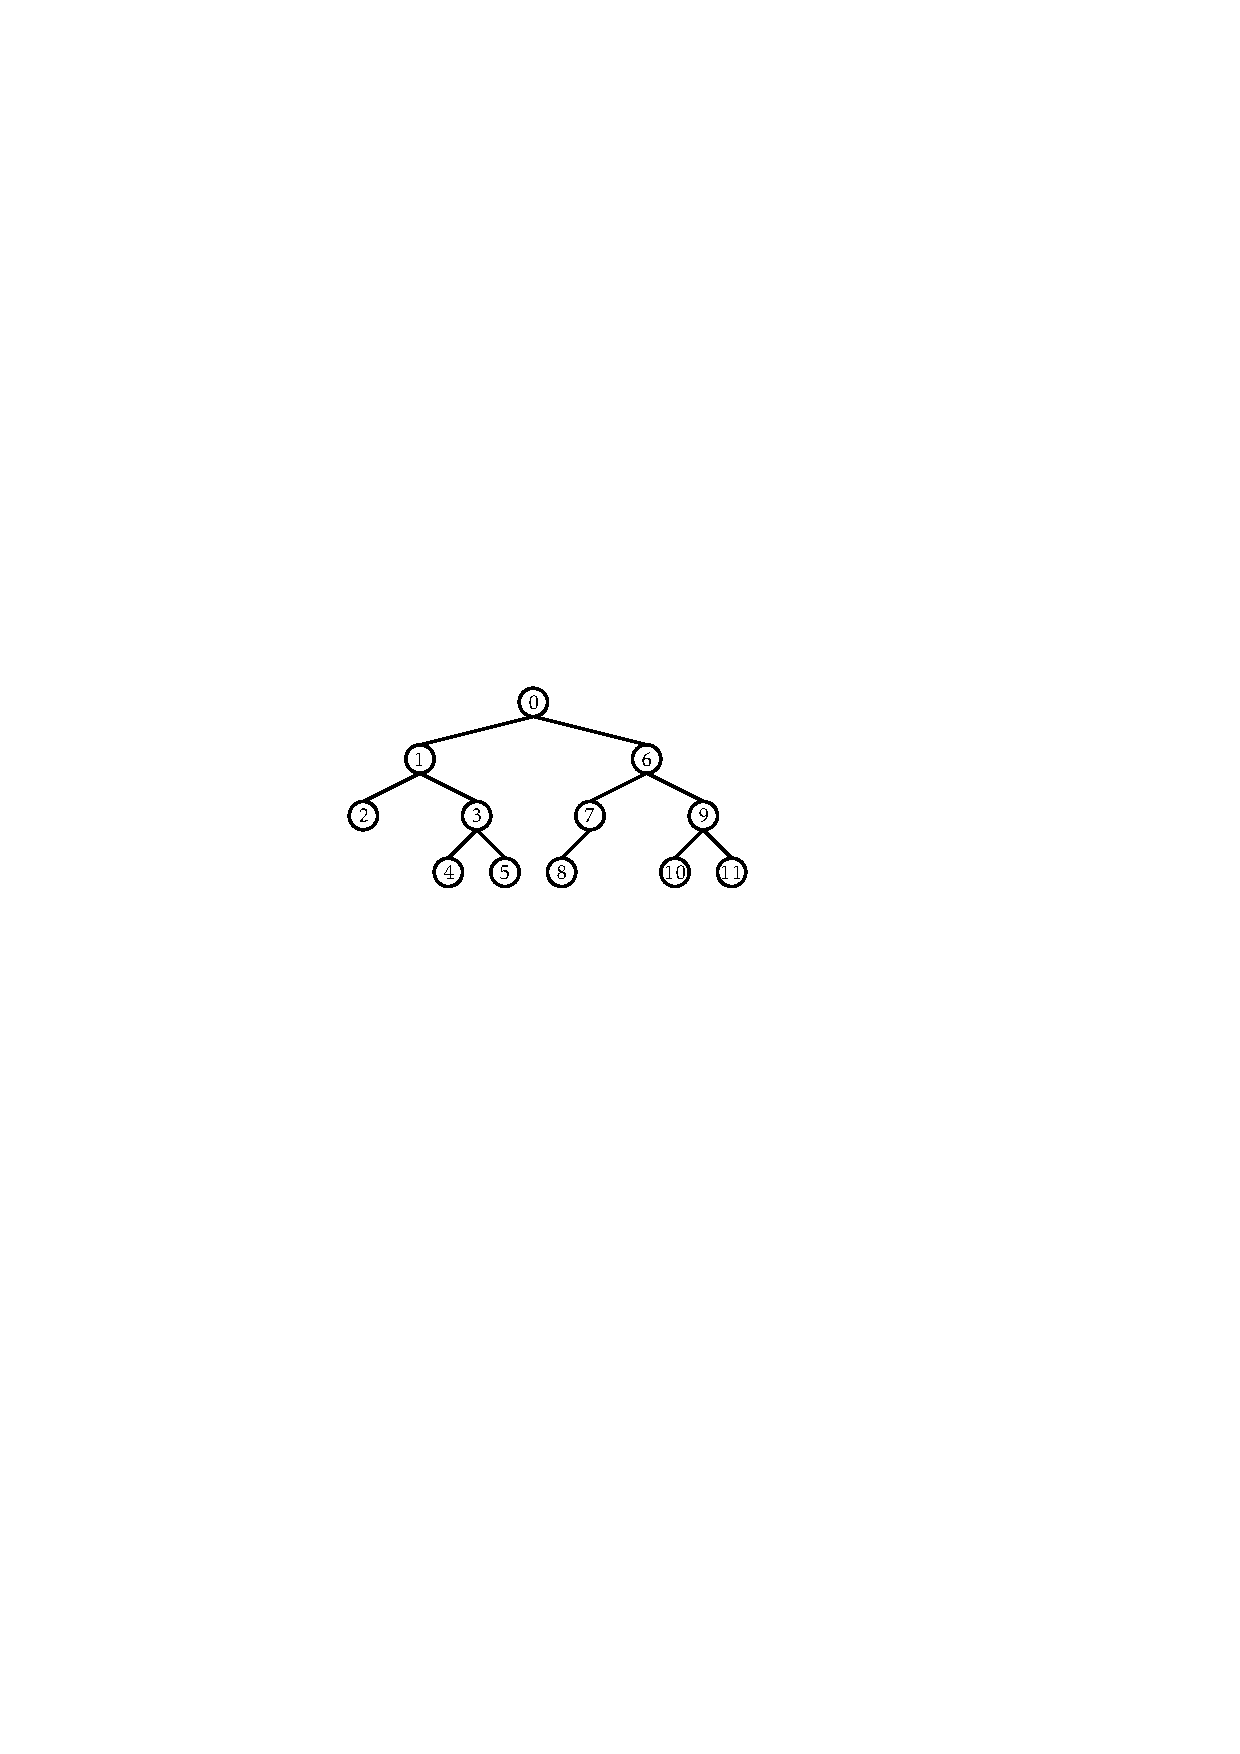
\includegraphics[scale=0.90909]{figs/binarytree-numbering-1}
    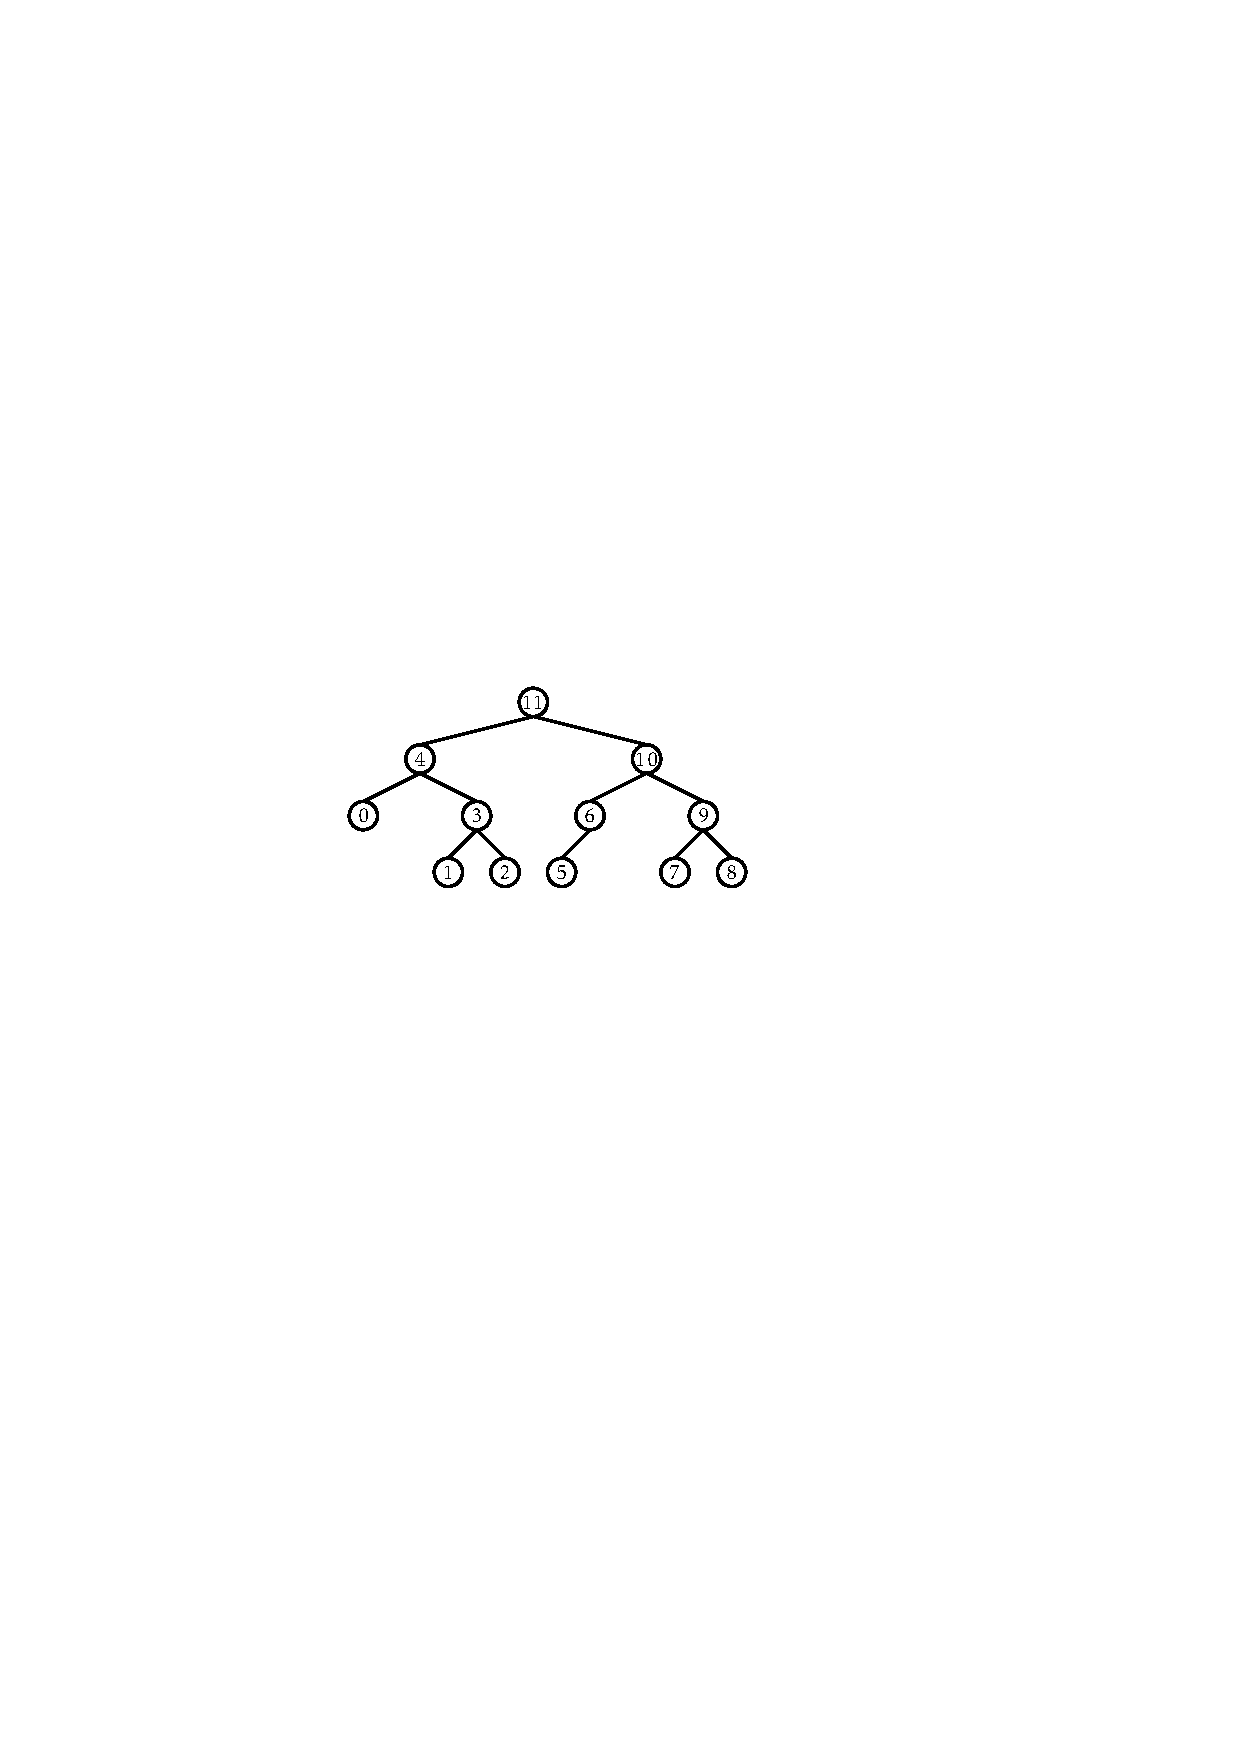
\includegraphics[scale=0.90909]{figs/binarytree-numbering-2} \\[2ex]
    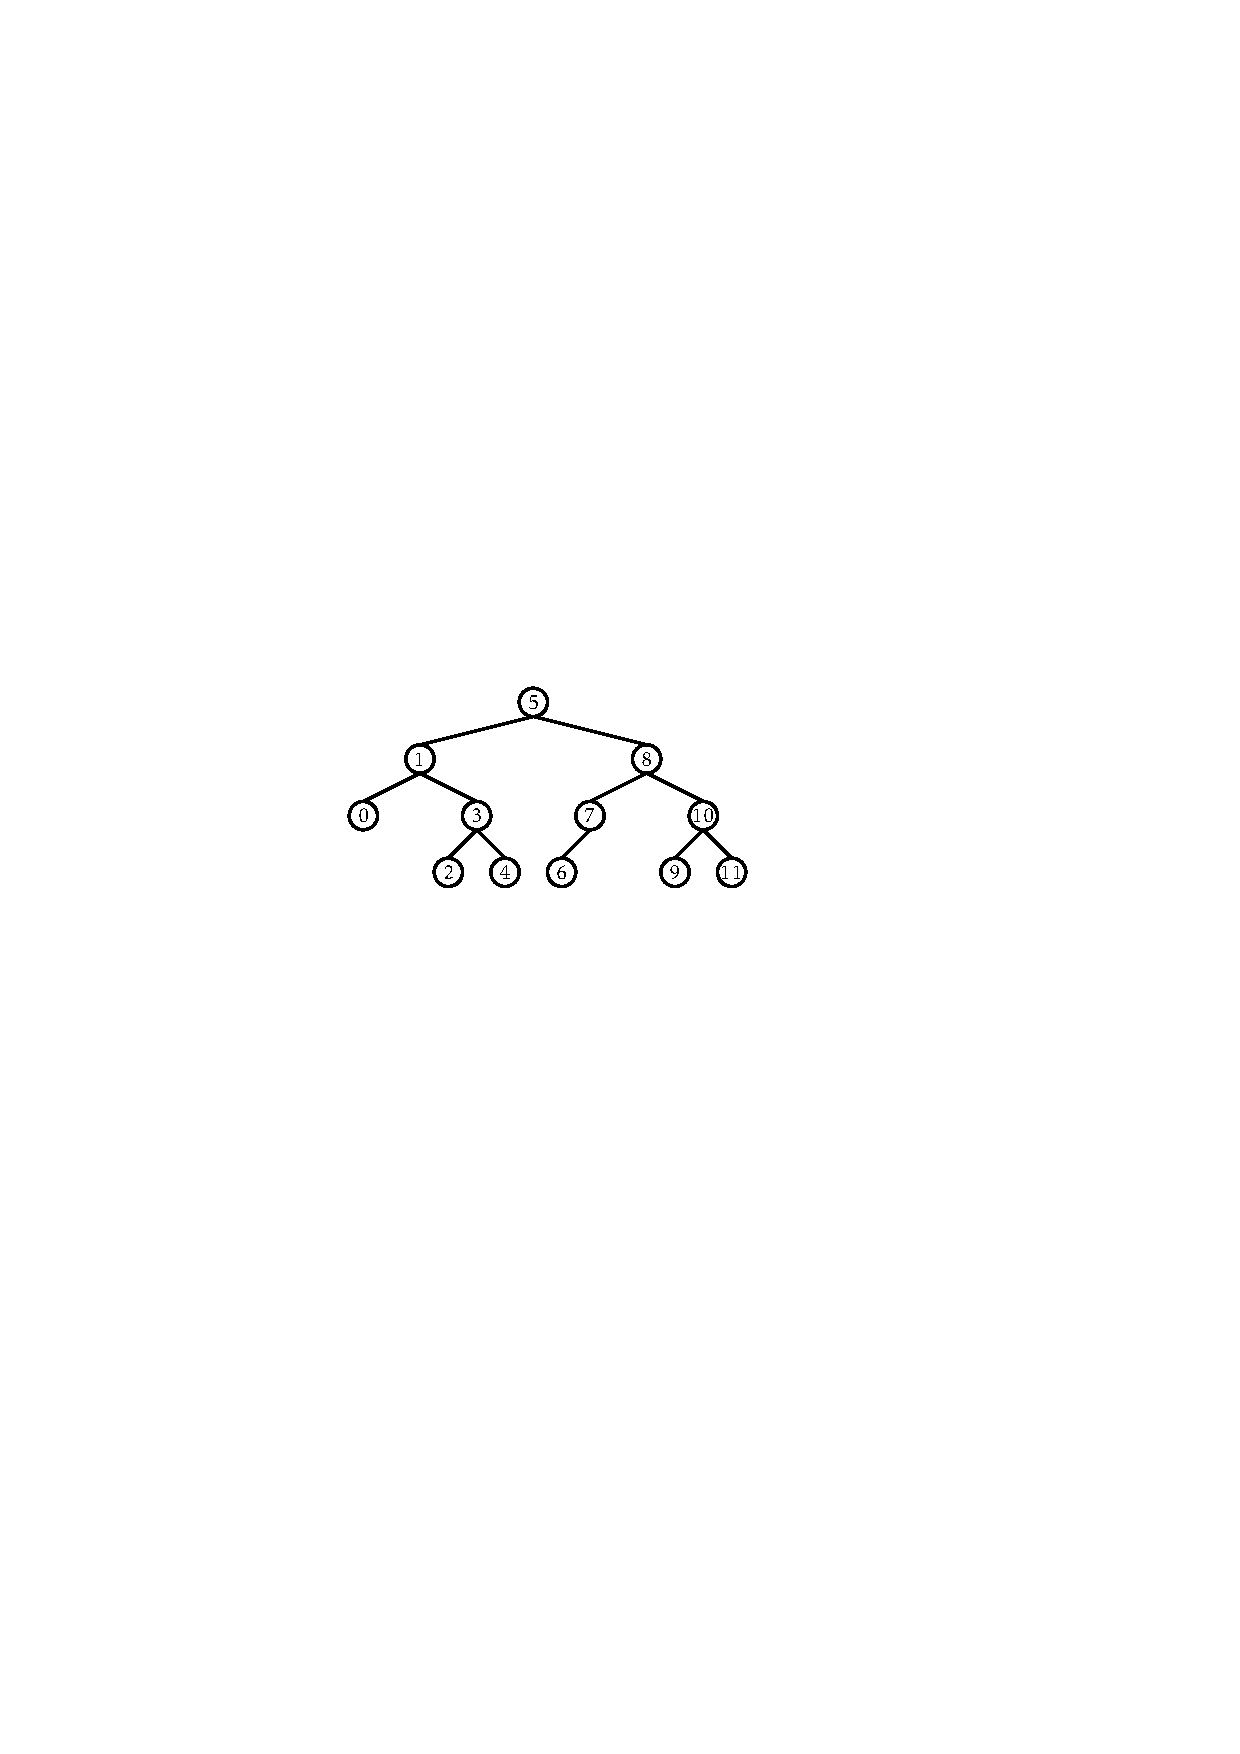
\includegraphics[scale=0.90909]{figs/binarytree-numbering-3}
  \end{center}
  \caption{Pre-order, post-order, and in-order numberings of a binary tree.}
  \figlabel{binarytree-numbering}
\end{figure}

\begin{exc}
  \index{number!pre-order}%
  \index{number!post-order}%
  \index{number!in-order}%
  \index{pre-order number}%
  \index{post-order number}%
  \index{in-order number}%
  Create a subclass of #BinaryTree# whose nodes have fields for storing
  pre-order, post-order, and in-order numbers.  Write recursive methods
  #preOrderNumber()#, #inOrderNumber()#, and #postOrderNumbers()# that
  assign these numbers correctly. These methods should each run in
  $O(#n#)$ time.
\end{exc}

\begin{exc}\exclabel{tree-traversal}
  Implement the non-recursive functions #nextPreOrder(u)#, #nextInOrder(u)#, and
  #nextPostOrder(u)# that return the node that follows #u# in a pre-order,
  in-order, or post-order traversal, respectively.   These functions
  should take amortized constant time; if we start at any node
  #u# and repeatedly call one of these functions and assign the return
  value to #u# until $#u#=#null#$, then the cost of all these calls should
  be $O(#n#)$.
\end{exc}

\begin{exc}
  Suppose we are given a binary tree with pre-, post-, and in-order numbers
  assigned to the nodes.  Show how these numbers can be used to answer
  each of the following questions in constant time:
  \begin{enumerate}
    \item Given a node #u#, determine the size of the subtree rooted at #u#.
    \item Given a node #u#, determine the depth of #u#.
    \item Given two nodes #u# and #w#, determine if #u# is an ancestor of #w#
  \end{enumerate}
\end{exc}

\begin{exc}
  Suppose you are given a list of nodes with pre-order and in-order
  numbers assigned.  Prove that there is at most one possible tree with
  this pre-order/in-order numbering and show how to construct it.
\end{exc}

\begin{exc}
  Show that the shape of any binary tree on #n# nodes can be represented
  using at most $2(#n#-1)$ bits.  (Hint: think about recording what
  happens during a traversal and then playing back that recording to
  reconstruct the tree.)
\end{exc}

\begin{exc}
  Illustrate what happens when we add the values $3.5$ and then 4.5 to
  the binary search tree in \figref{bst}.
\end{exc}

\begin{exc}
  Illustrate what happens when we remove the values $3$ and then 5 from
  the binary search tree in \figref{bst}.
\end{exc}

\begin{exc}
  Implement a #BinarySearchTree# method, #getLE(x)#,
  that returns a list of all items in the tree that are less than or
  equal to #x#.  The running time of your method should be $O(#n#'+#h#)$
  where $#n#'$ is the number of items less than or equal to #x# and #h#
  is the height of the tree.
\end{exc}

\begin{exc}
  Describe how to add the elements $\{1,\ldots,#n#\}$ to an initially
  empty #BinarySearchTree# in such a way that the resulting tree has
  height $#n#-1$.  How many ways are there to do this?
\end{exc}

\begin{exc}
  If we have some #BinarySearchTree# and perform the operations #add(x)#
  followed by #remove(x)# (with the same value of #x#) do we necessarily
  return to the original tree?
\end{exc}

\begin{exc}
  Can a #remove(x)# operation increase the height of any node in a
  #BinarySearchTree#?  If so, by how much?
\end{exc}

\begin{exc}
  Can an #add(x)# operation increase the height of any node in a
  #BinarySearchTree#?  Can it increase the height of the tree?  If so,
  by how much?
\end{exc}

\begin{exc}
  Design and implement a version of #BinarySearchTree# in which each node,
  #u#, maintains values #u.size# (the size of the subtree rooted at #u#),
  #u.depth# (the depth of #u#), and #u.height# (the height of the subtree
  rooted at #u#).  

  These values should be maintained, even during calls to the #add(x)#
  and #remove(x)# operations, but this should not increase the cost of
  these operations by more than a constant factor.
\end{exc}
